% 第5章 实验结果
% 图均为 v3 冻结设计（快照 20261012T0033Z-full）下真实数据生成，哈希核验见
%   tcad-research-training/shared/evidence/reuse-audit-20261116.json 与 materials/图表引用清单.md
% 红线：失败与未决必须出现；配对≠独立事件；不把波形叫实测截面；新 r0.6 结果合格后按 5.7 节补入
\section{实验结果}

本章结果均来自 v3 冻结设计（64 个独立事件 / 128 条 bit0/1 配对响应，数据版本 20261012T0033Z-full），在未校准二维代表模型、固定 5\,MeV 粒子、两种角度与固定入射位置的范围内解释；r0.6 新结果合格后补入 5.7 节。

\subsection{初态与无粒子基线}

图\ref{fig:initial-state} 展示写入后的初态检查，是全部匹配对照的共同起点。8/8 无粒子物理/离线参考一致性已通过，各侧 4\ns 电压差绝对值最大约 $6\times10^{-15}\V$，三阈值分类一致。

\begin{figure}[htbp]
\centering
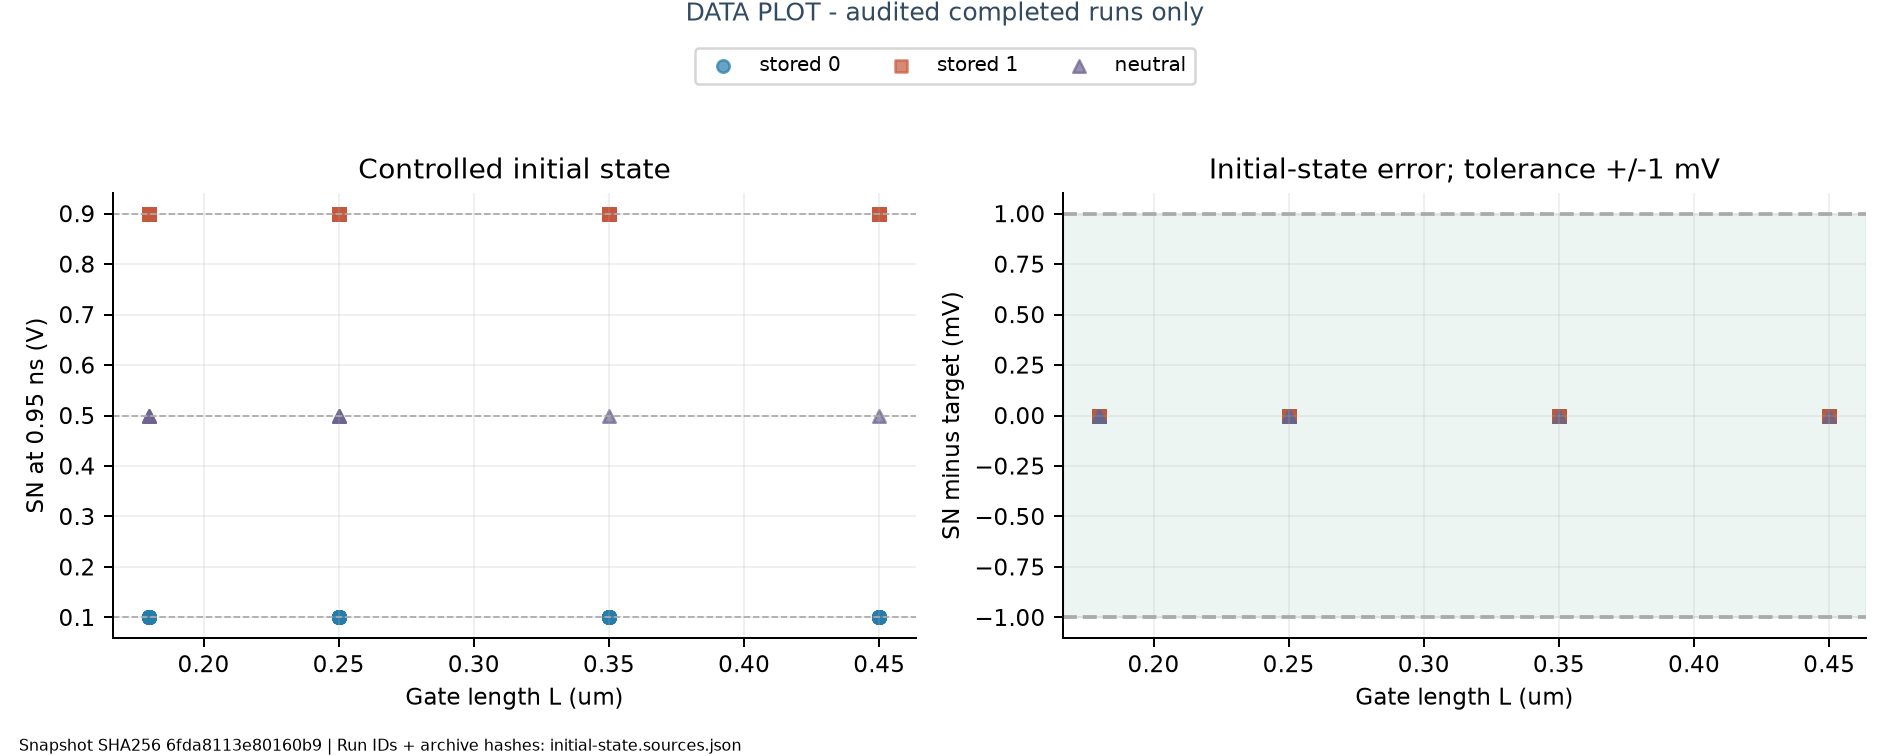
\includegraphics[width=0.8\textwidth]{figures/initial-state.png}
\caption{v3冻结设计下的写入初态检查。数据版本：20261012T0033Z-full；原始 run 与输入/输出哈希见共享证据索引。结果用于未校准代表模型的方法验证；v3 原结构与原时序，不代表真实 DDR5 校准。}
\label{fig:initial-state}
\end{figure}

\subsection{单粒子读出响应与多尺寸比较}

图\ref{fig:readout-l018}--\ref{fig:readout-l045} 给出四种栅长下相同事件/bit/对照的波形与读出裕量。固定 5\,MeV、固定入射位置与原二维代表模型；判据误读不等于持久位翻转。

\begin{figure}[htbp]
\centering
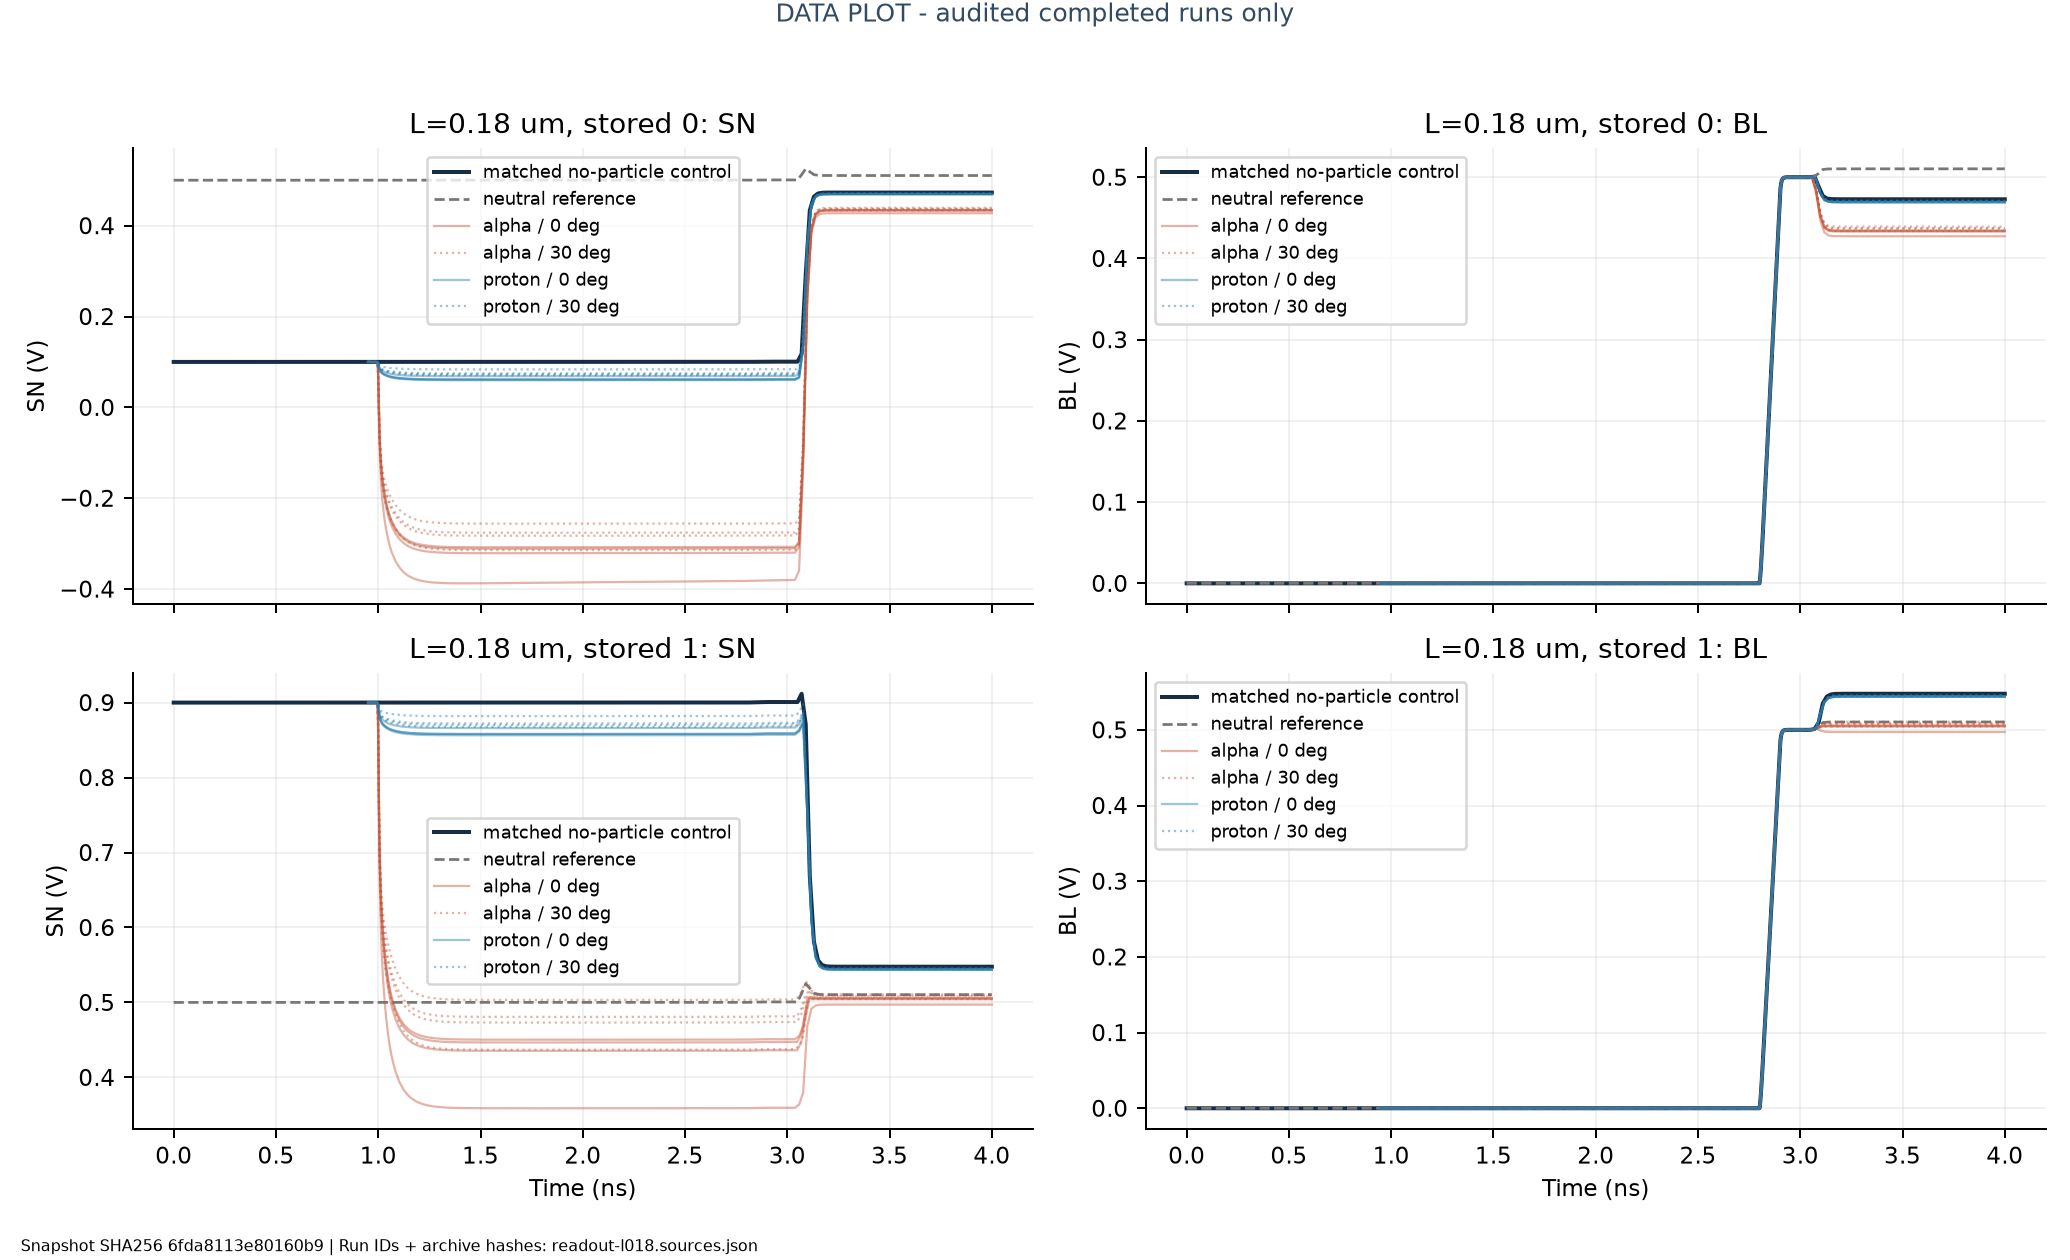
\includegraphics[width=0.48\textwidth]{figures/readout-l018.png}
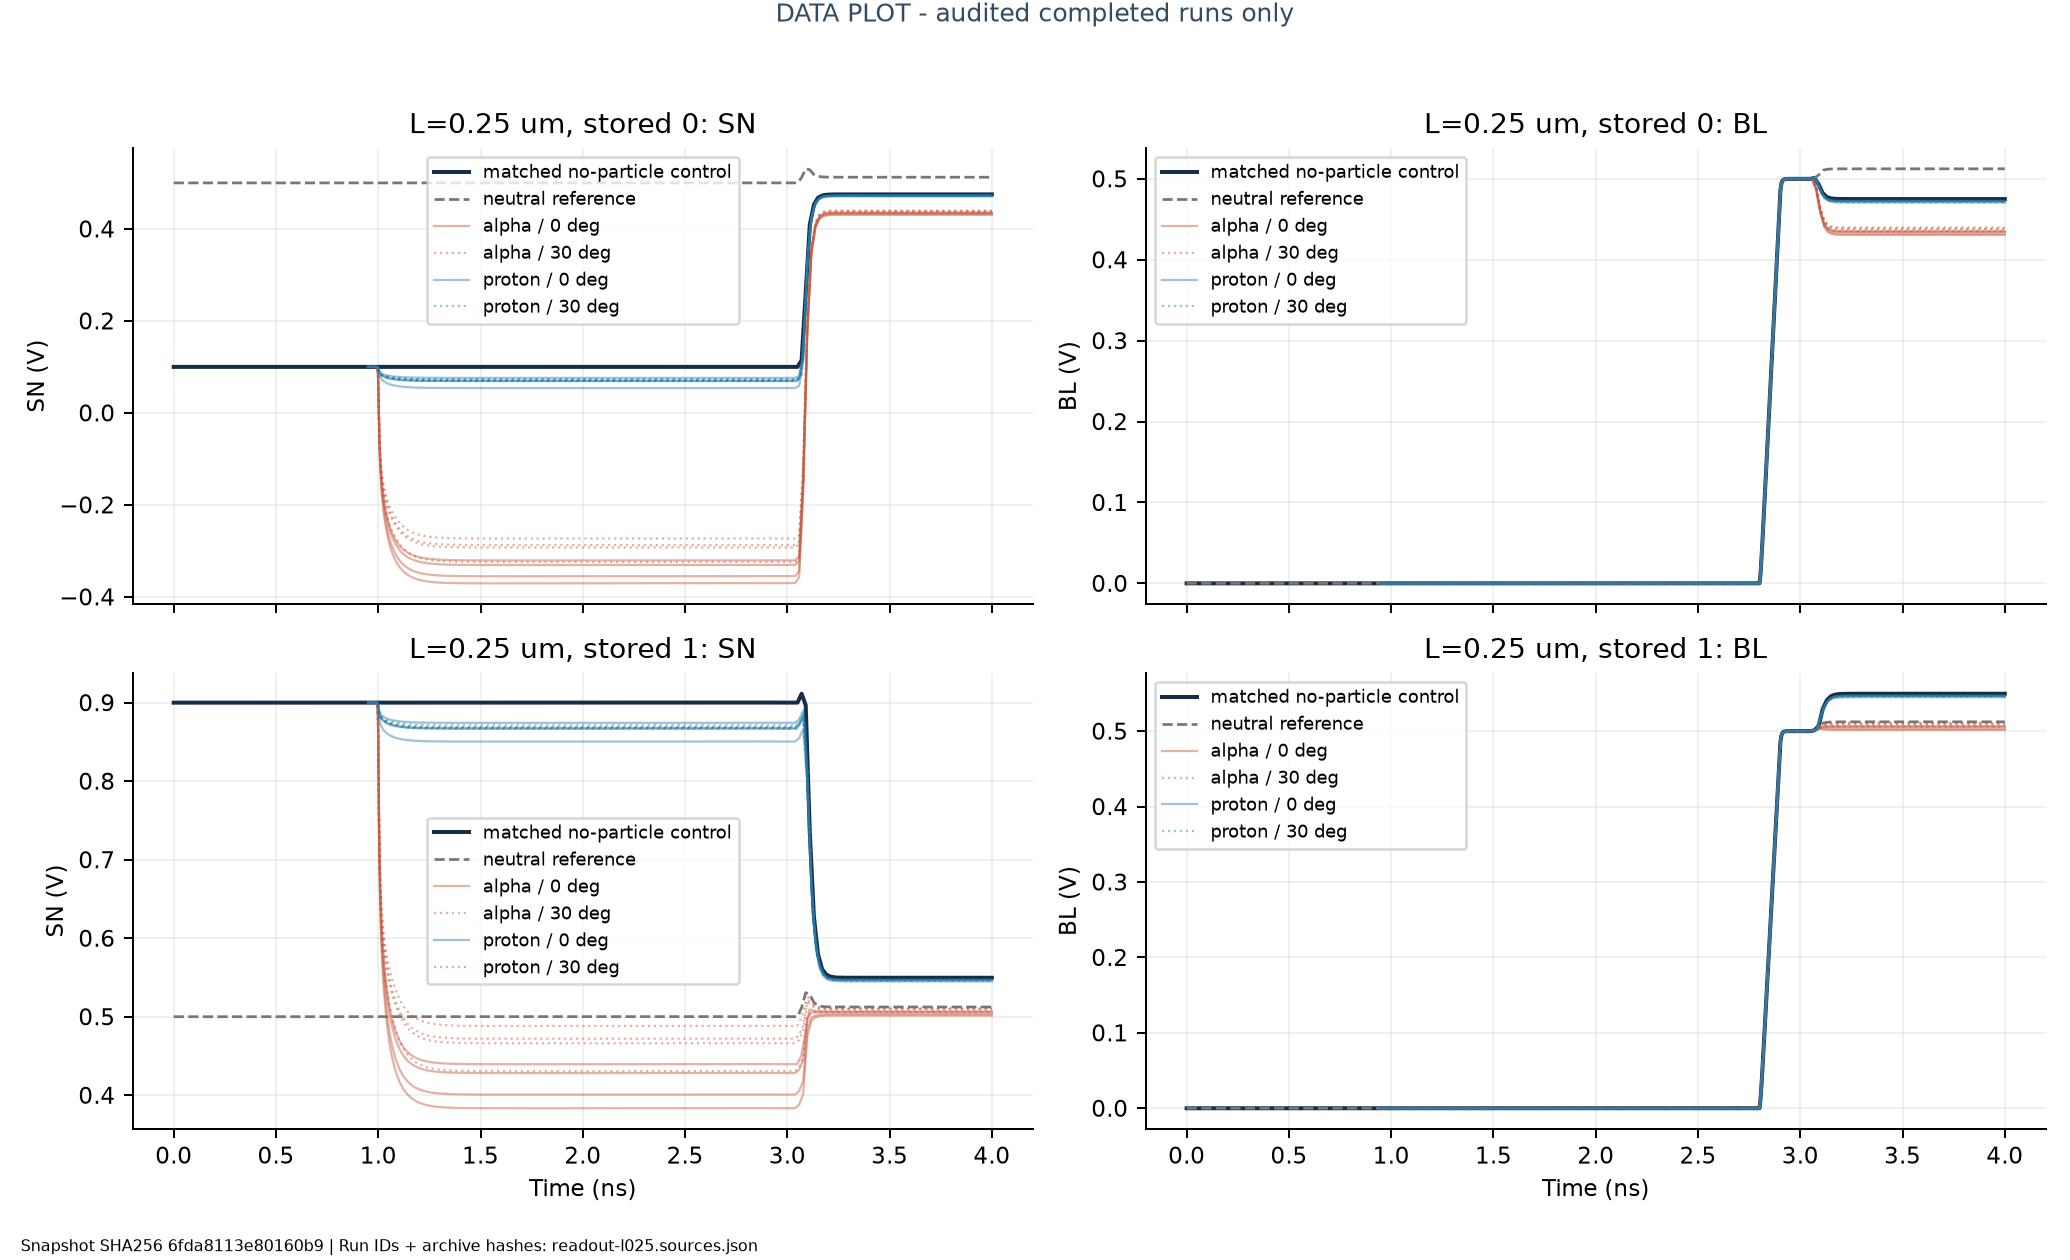
\includegraphics[width=0.48\textwidth]{figures/readout-l025.png}
\caption{v3冻结设计下 0.18/0.25\um 读出响应波形。数据版本：20261012T0033Z-full；固定 5\,MeV、固定位置、原二维代表模型。}
\label{fig:readout-l018}
\end{figure}
\begin{figure}[htbp]
\centering
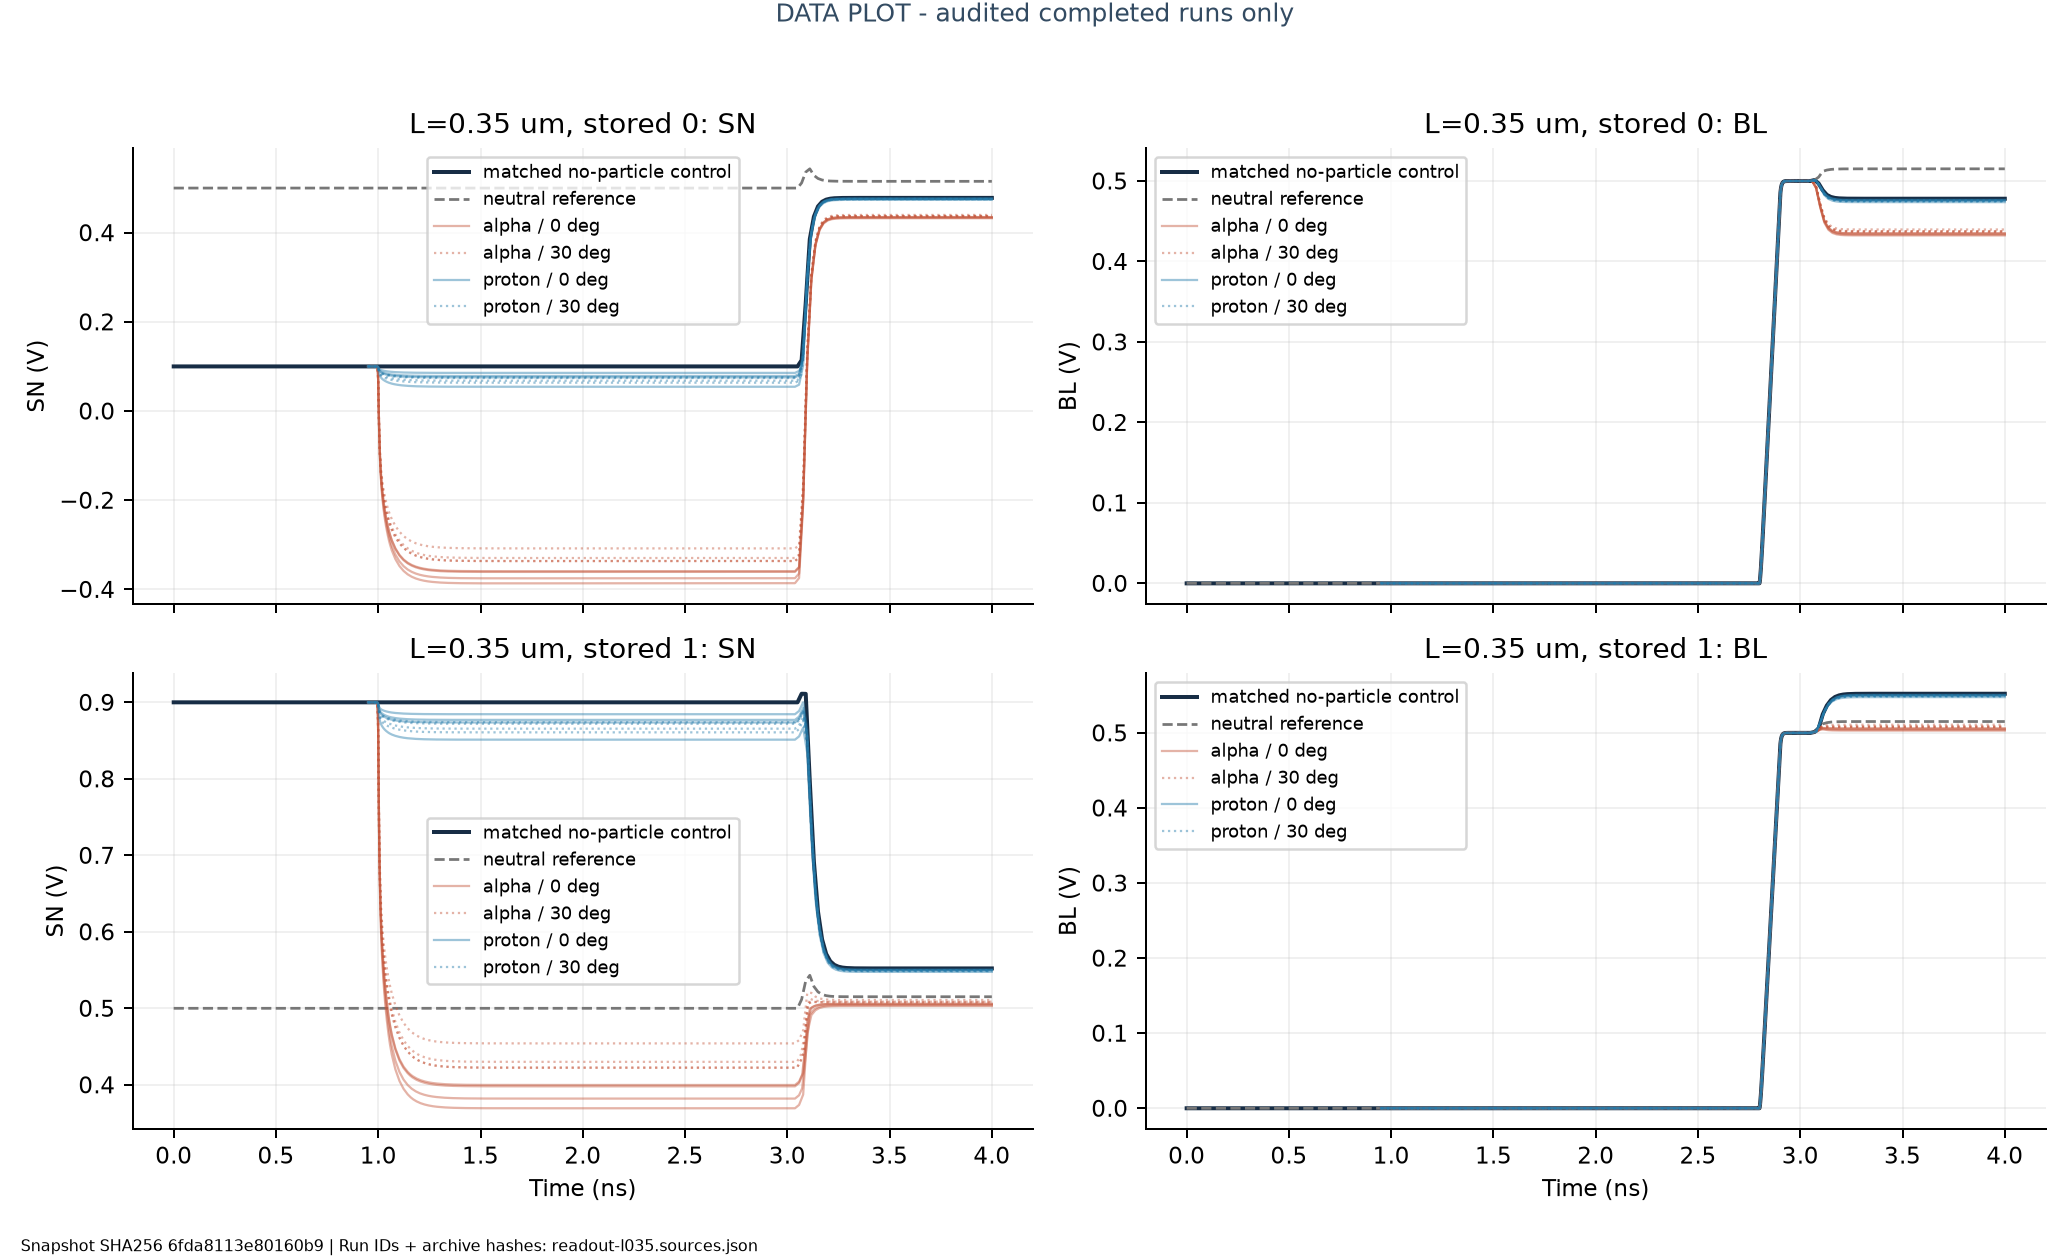
\includegraphics[width=0.48\textwidth]{figures/readout-l035.png}
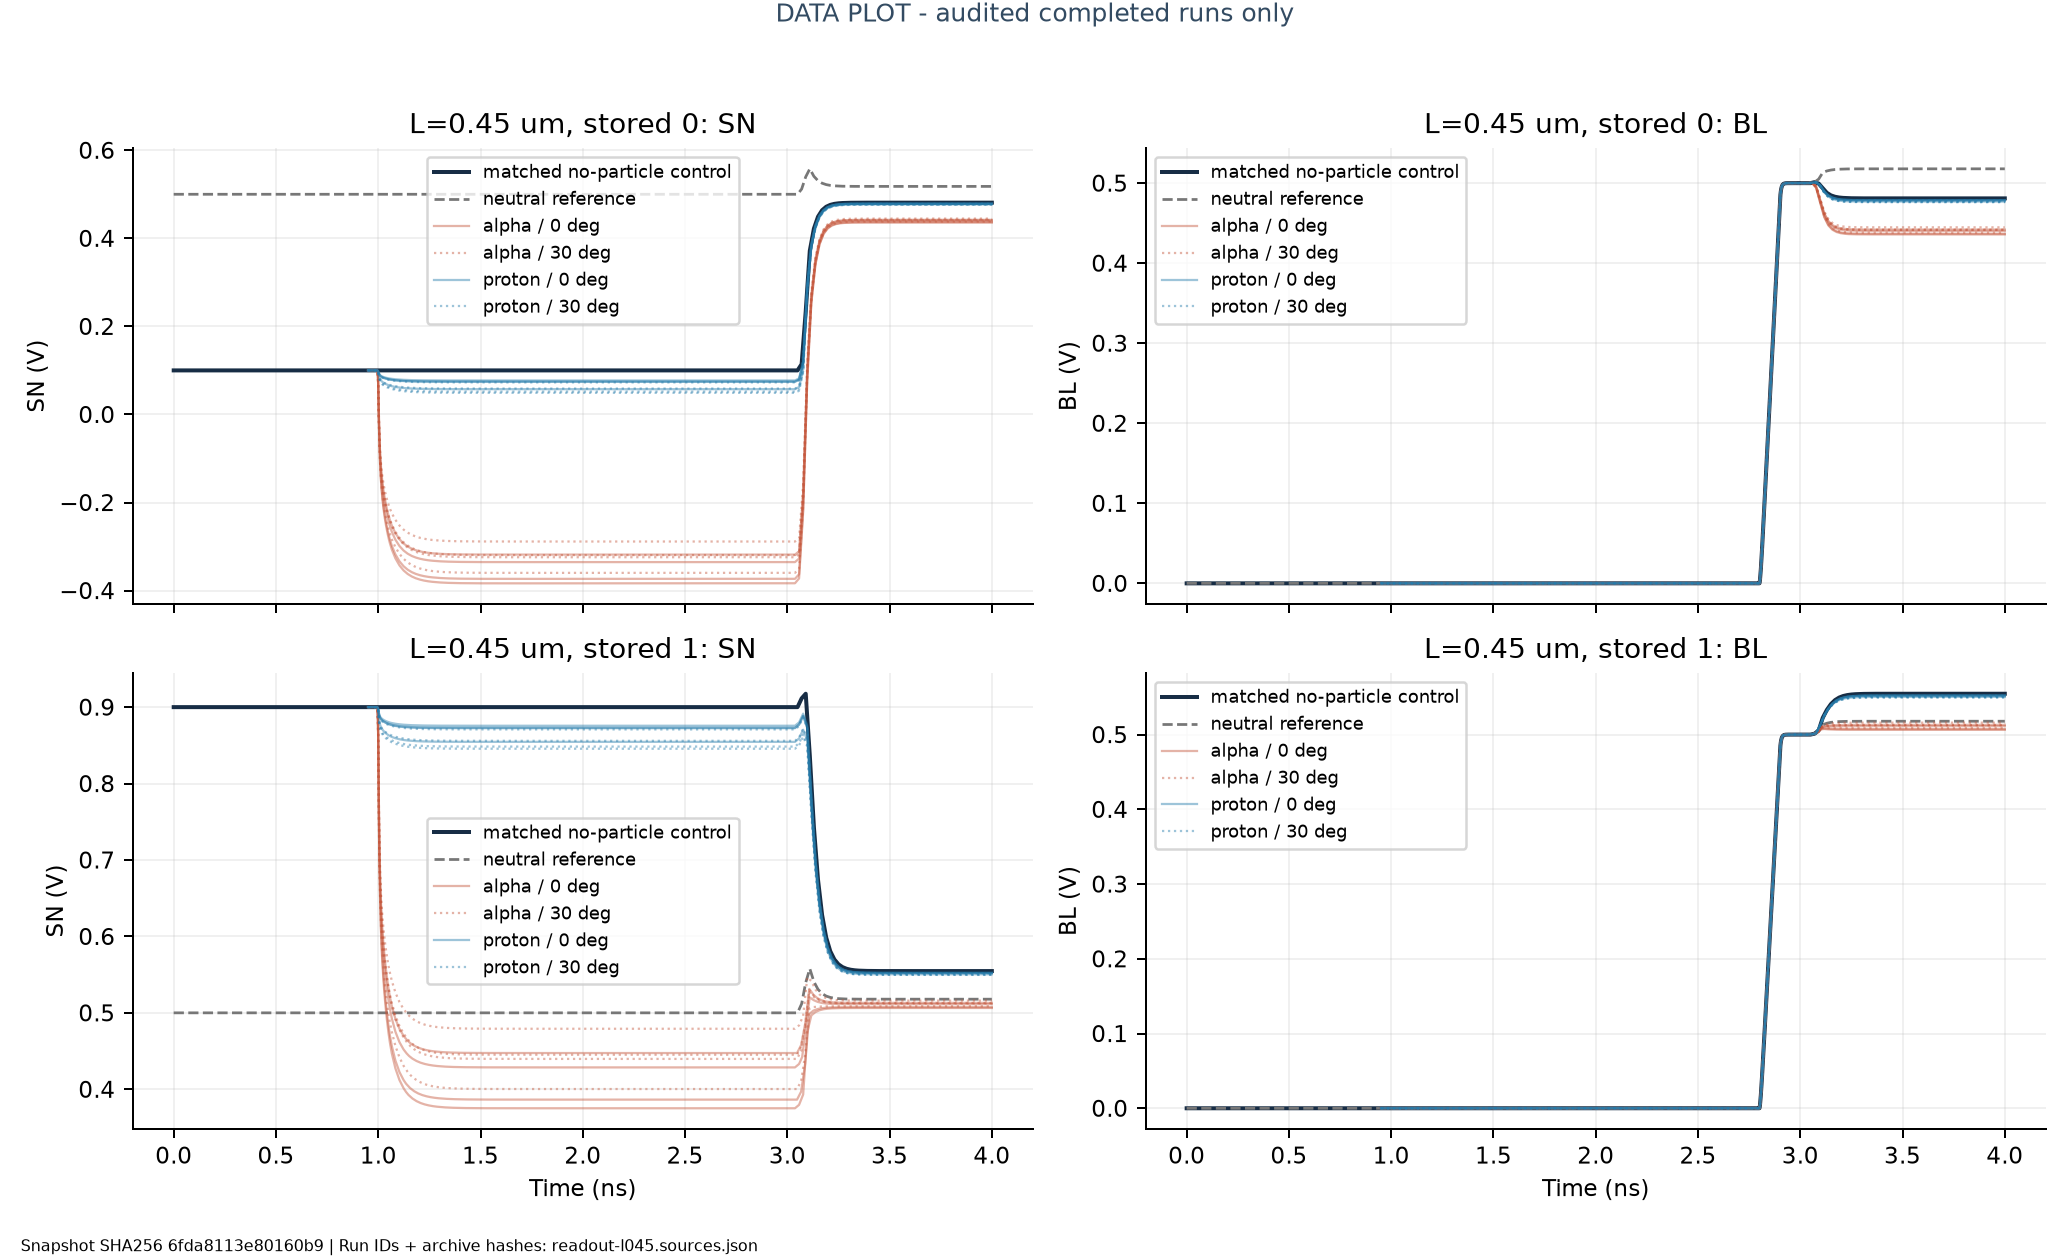
\includegraphics[width=0.48\textwidth]{figures/readout-l045.png}
\caption{v3冻结设计下 0.35/0.45\um 读出响应波形。数据版本：20261012T0033Z-full；误读不等于持久翻转。}
\label{fig:readout-l045}
\end{figure}

\subsection{分类统计与不确定性}

5\mV 主阈值下 128 条配对响应分类为 96 正确、20 判据误读、8 临界、4 数值不确定（图\ref{fig:stratum-counts}）；临界与数值不确定不并入正确，也不改写为已证翻转。图\ref{fig:stratum-intervals} 给出分层统计区间：每物理条件每 bit 的计划独立事件 $N=4$，不是截面，也不是同时覆盖所有分层的 95\% 区间。

\begin{figure}[htbp]
\centering
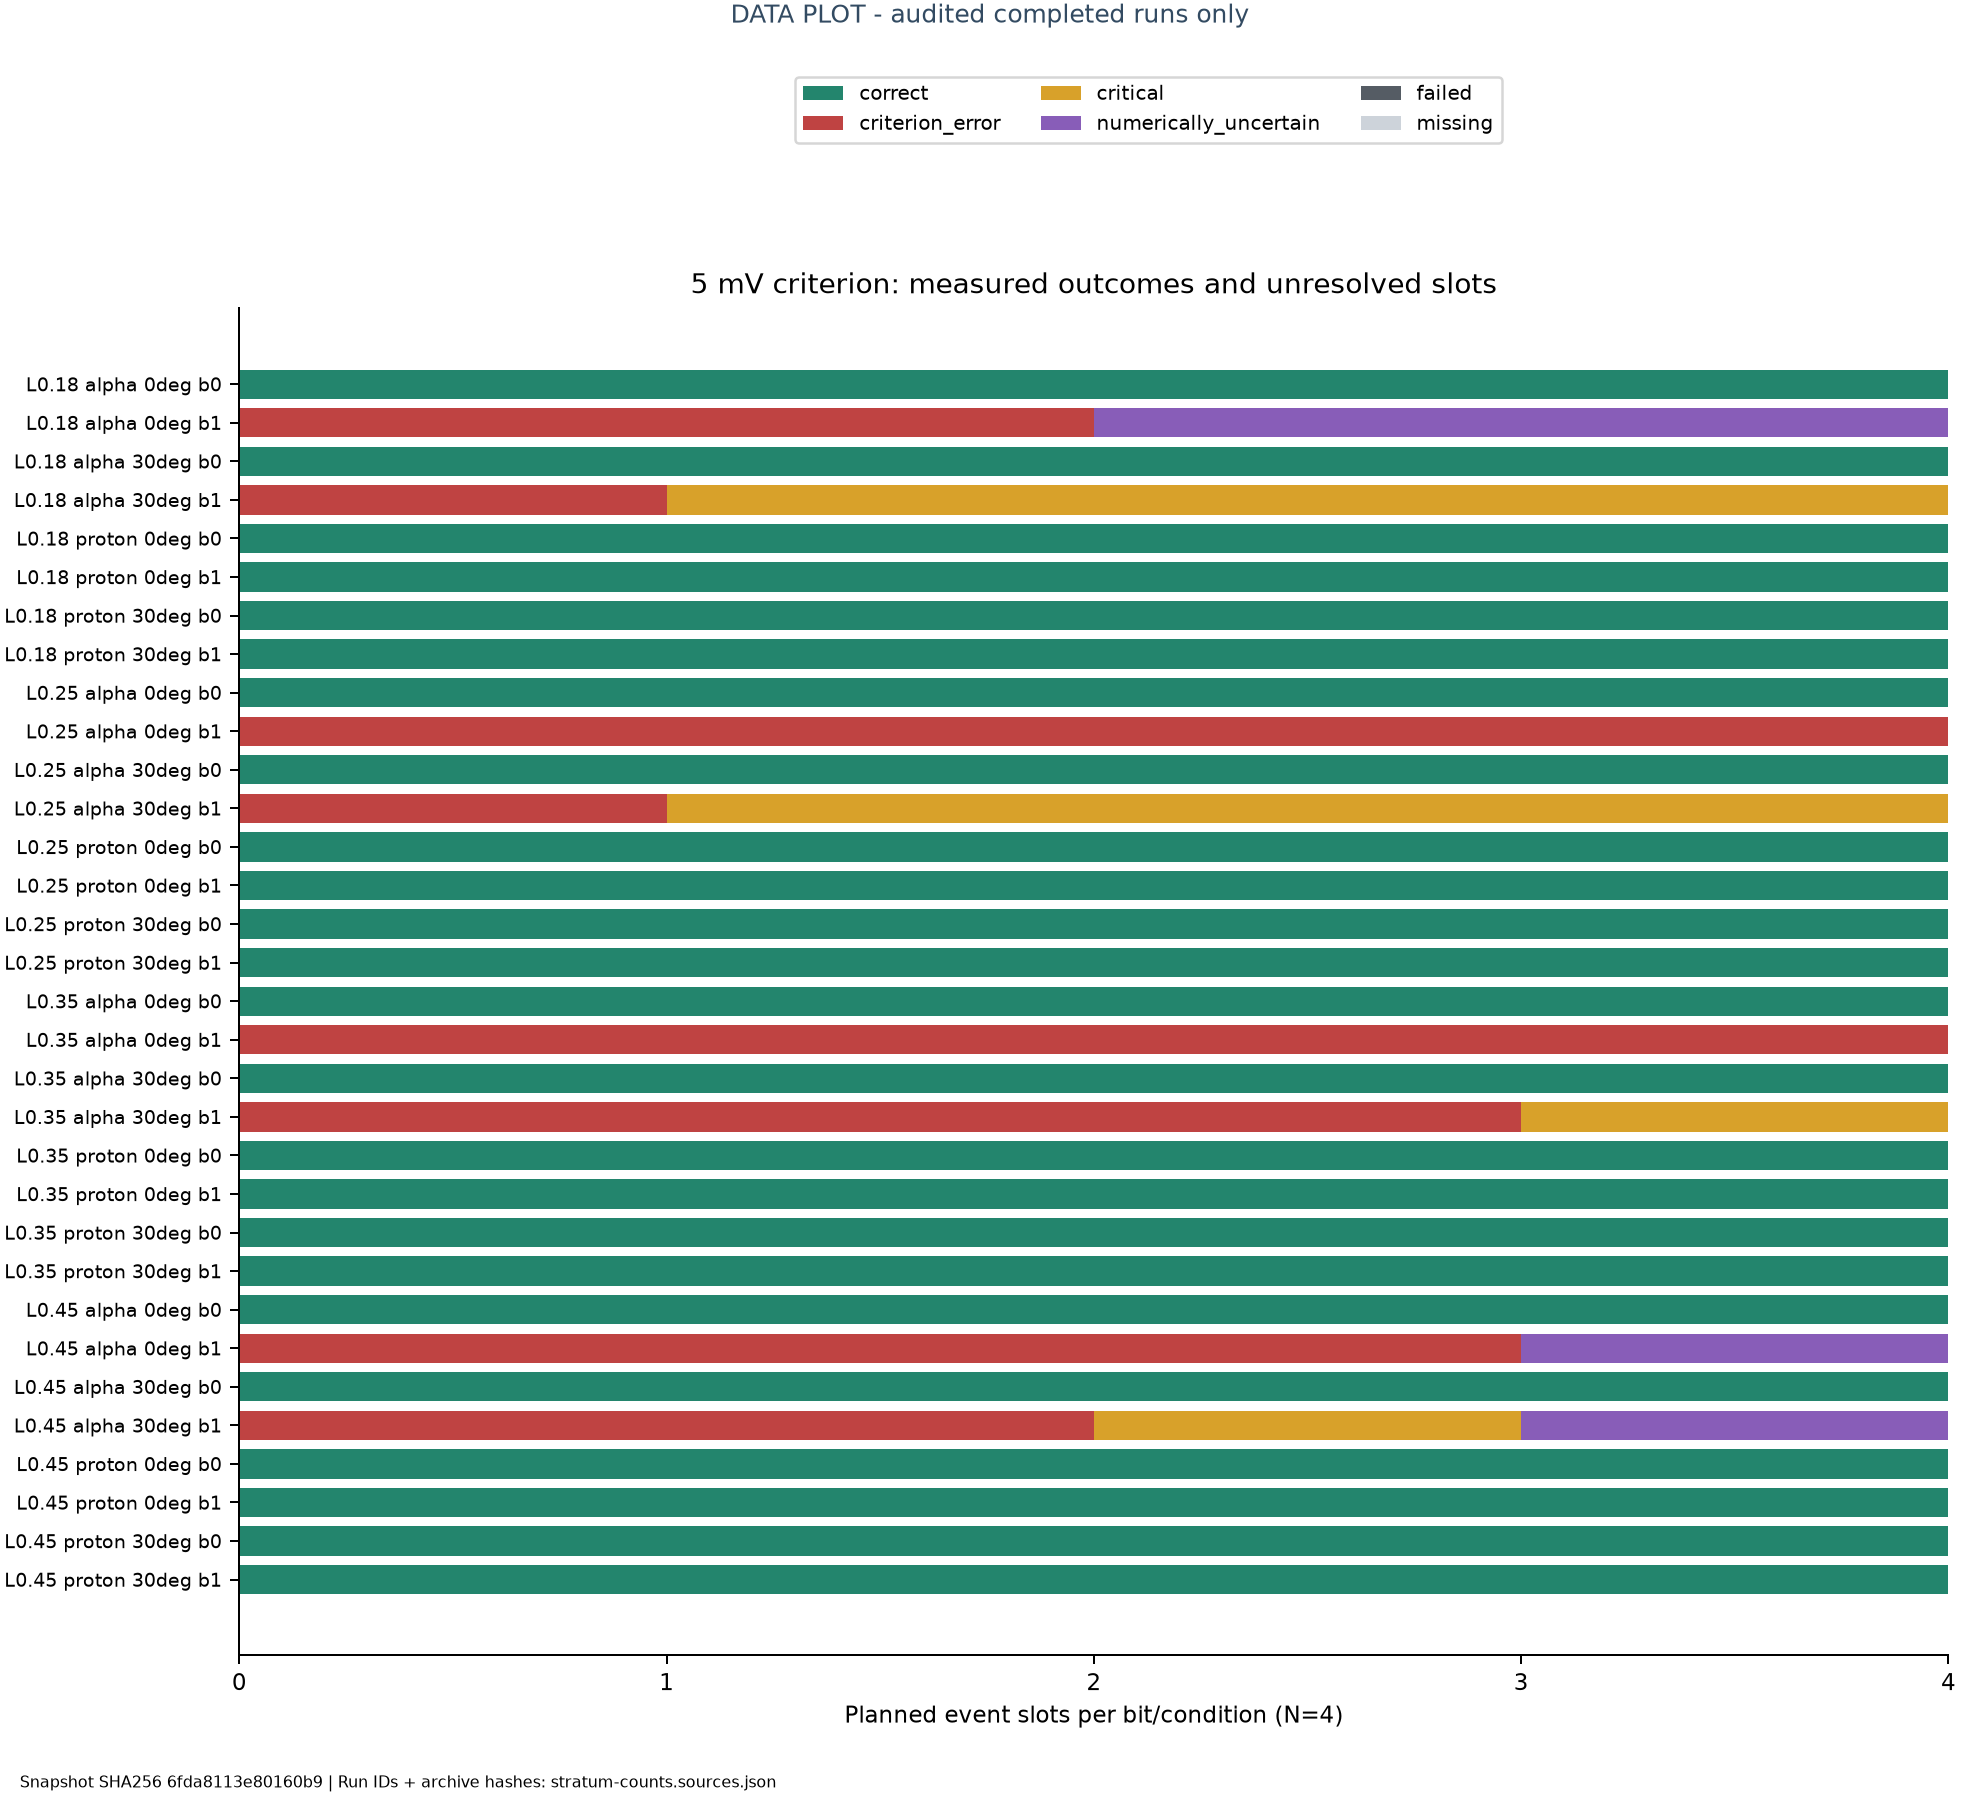
\includegraphics[width=0.7\textwidth]{figures/stratum-counts.png}
\caption{v3冻结设计下主阈值分类计数（正确/误读/临界/数值不确定），共 64 独立事件/128 配对响应，不删除未决。数据版本：20261012T0033Z-full。}
\label{fig:stratum-counts}
\end{figure}
\begin{figure}[htbp]
\centering
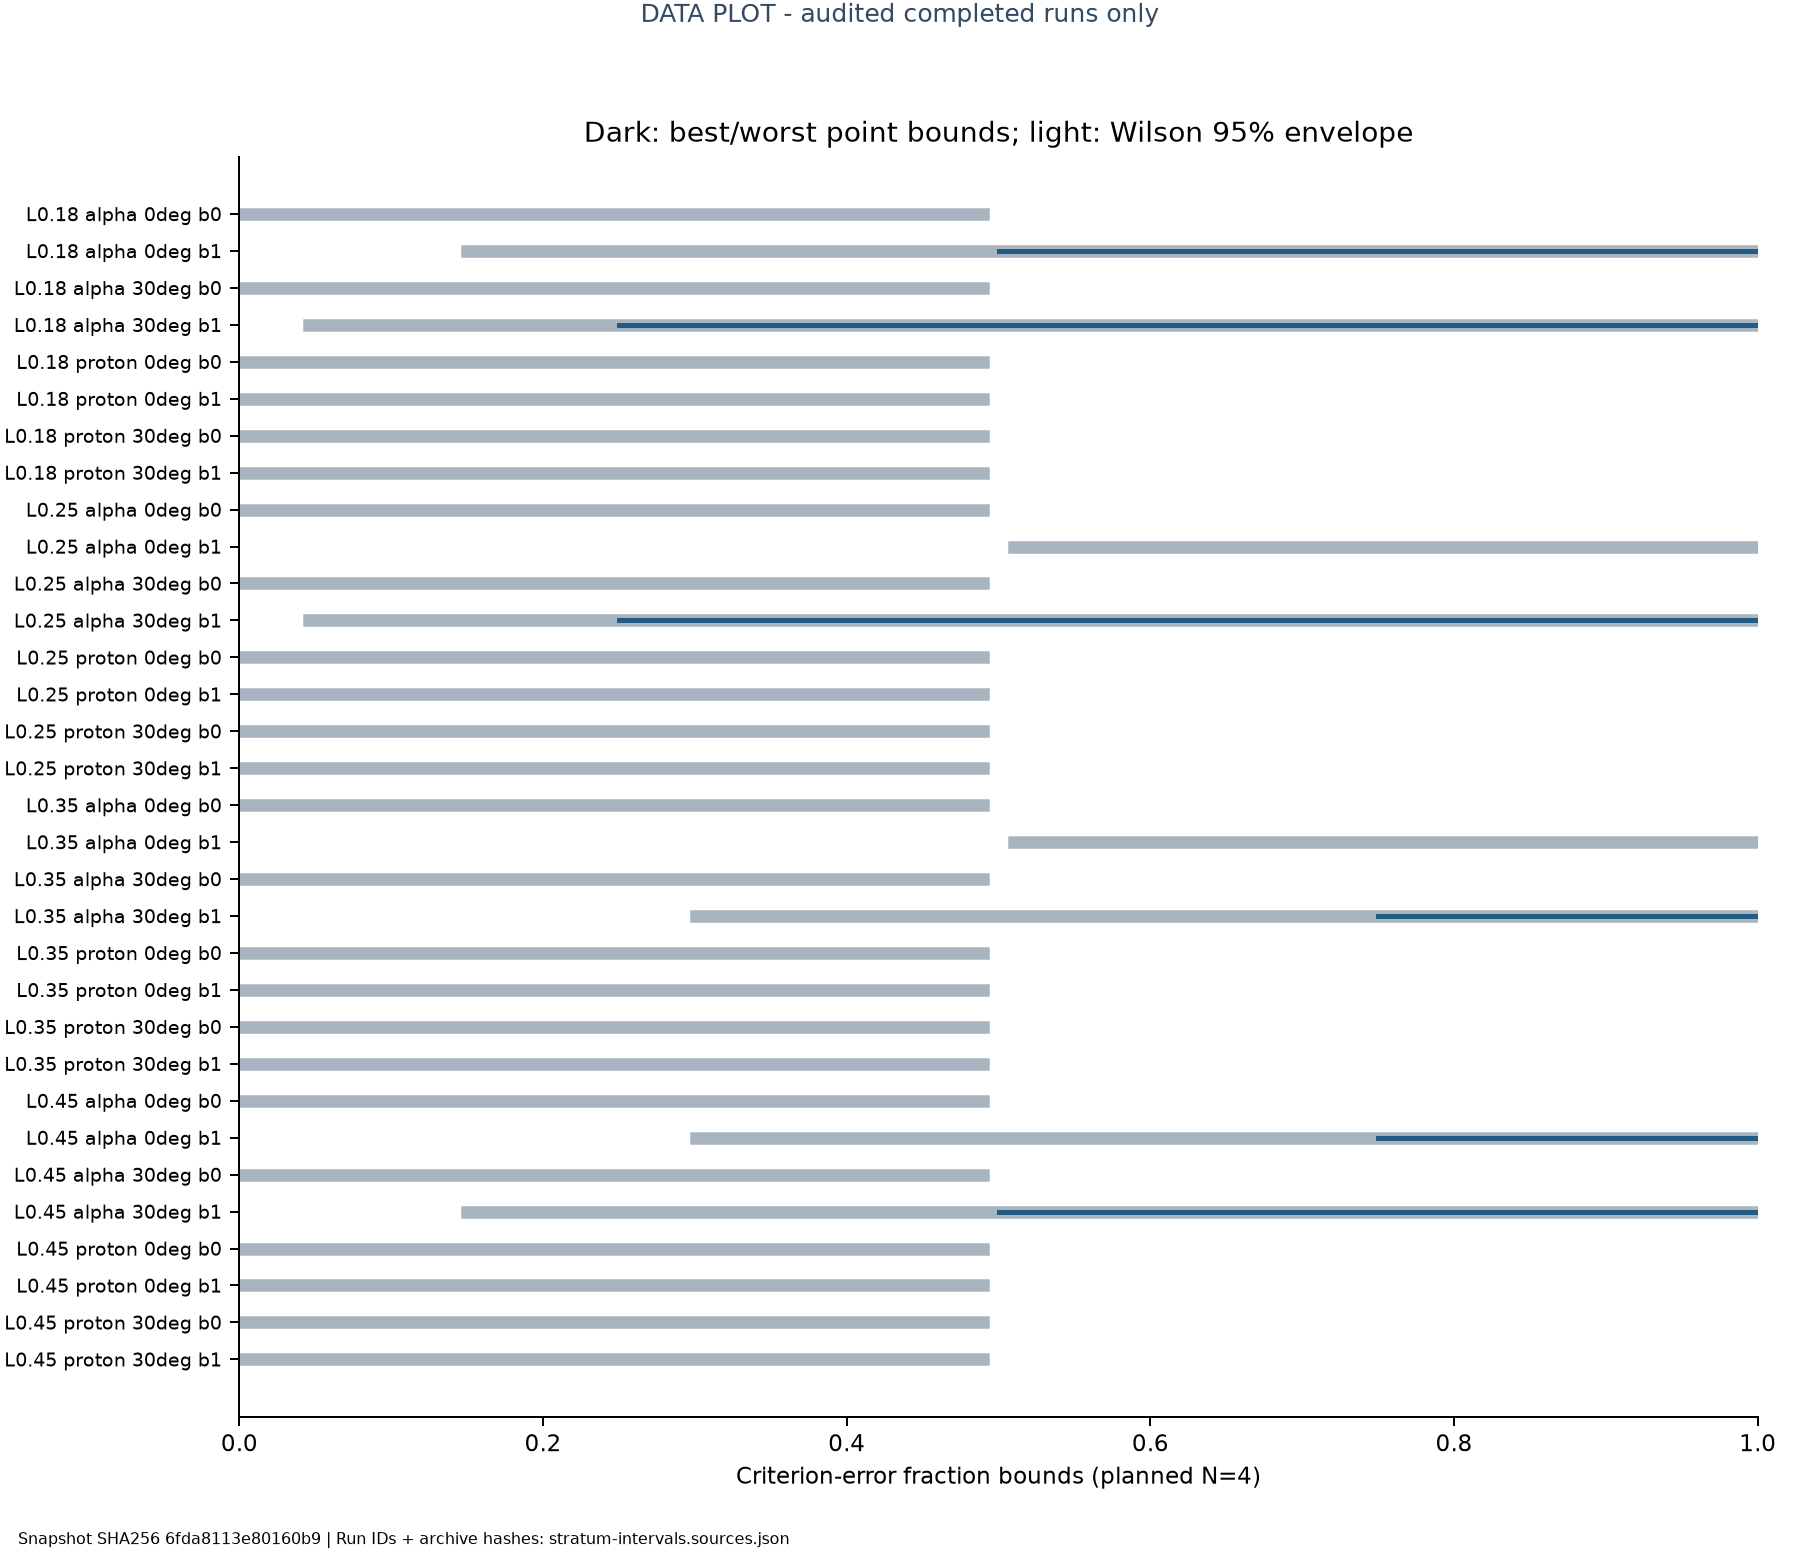
\includegraphics[width=0.7\textwidth]{figures/stratum-intervals.png}
\caption{v3冻结设计下分层统计区间（小样本与未决带来的不确定性）；每条件每 bit $N=4$，不是截面。数据版本：20261012T0033Z-full。}
\label{fig:stratum-intervals}
\end{figure}

\subsection{阈值与读窗敏感性}

图\ref{fig:threshold-l018}--\ref{fig:threshold-l045} 展示 2.5/5/10\mV 阈值与 3.8--4\ns 读窗敏感性；4\ns 单点分类与整个读窗稳定性分开报告。

\begin{figure}[htbp]
\centering
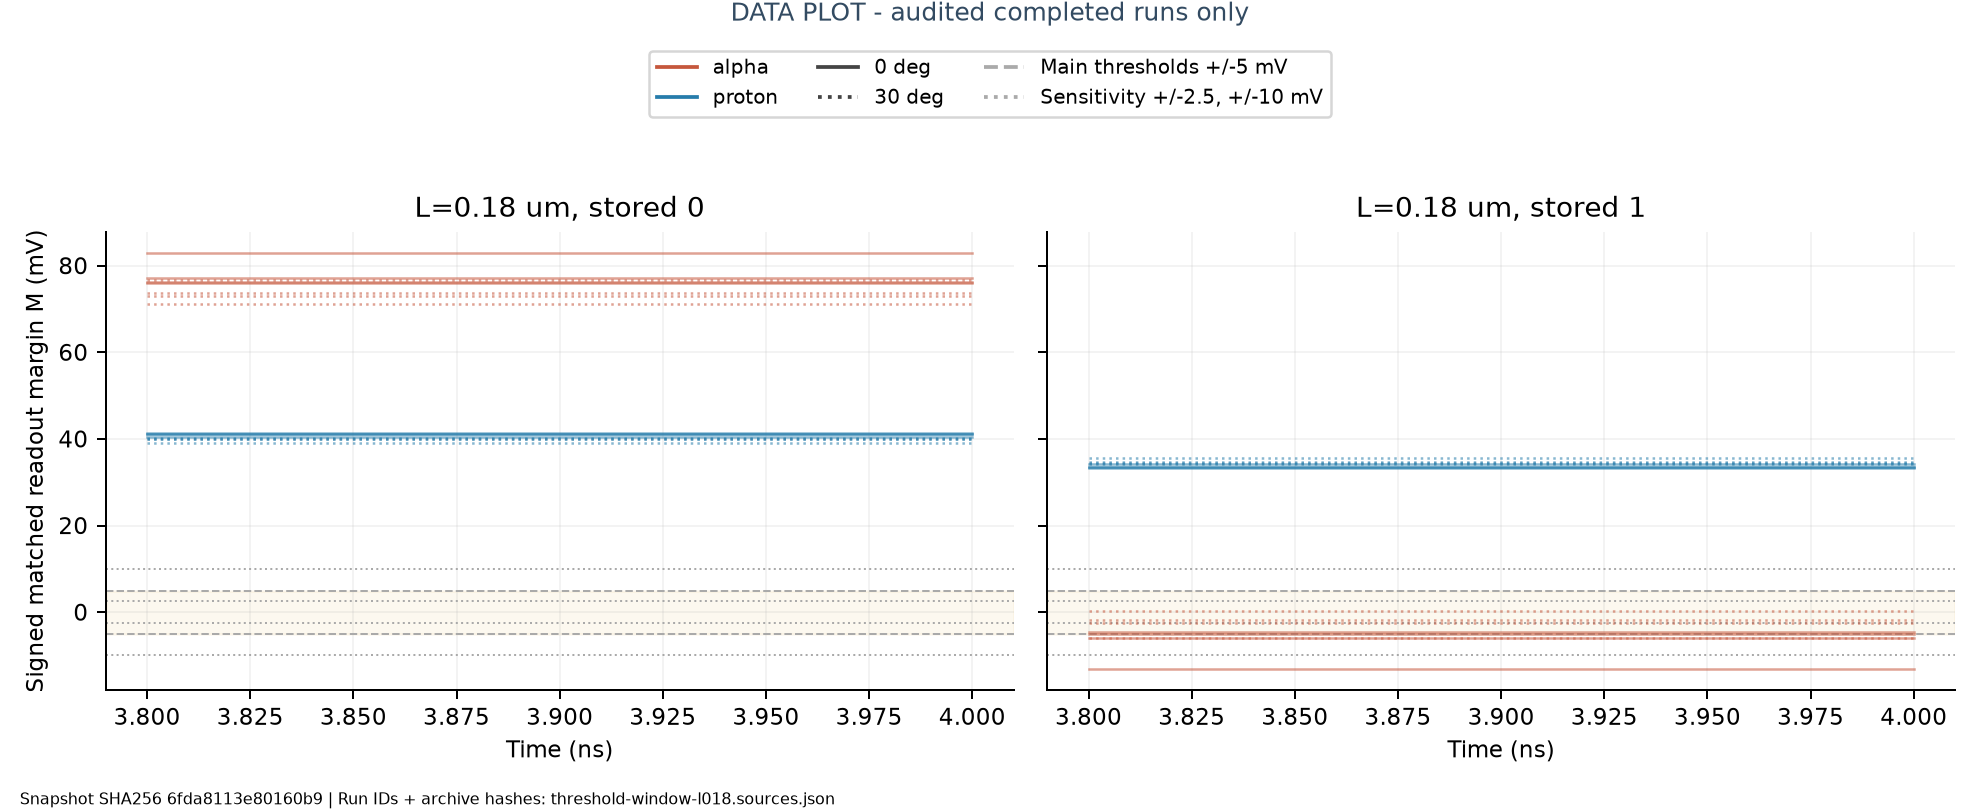
\includegraphics[width=0.48\textwidth]{figures/threshold-window-l018.png}
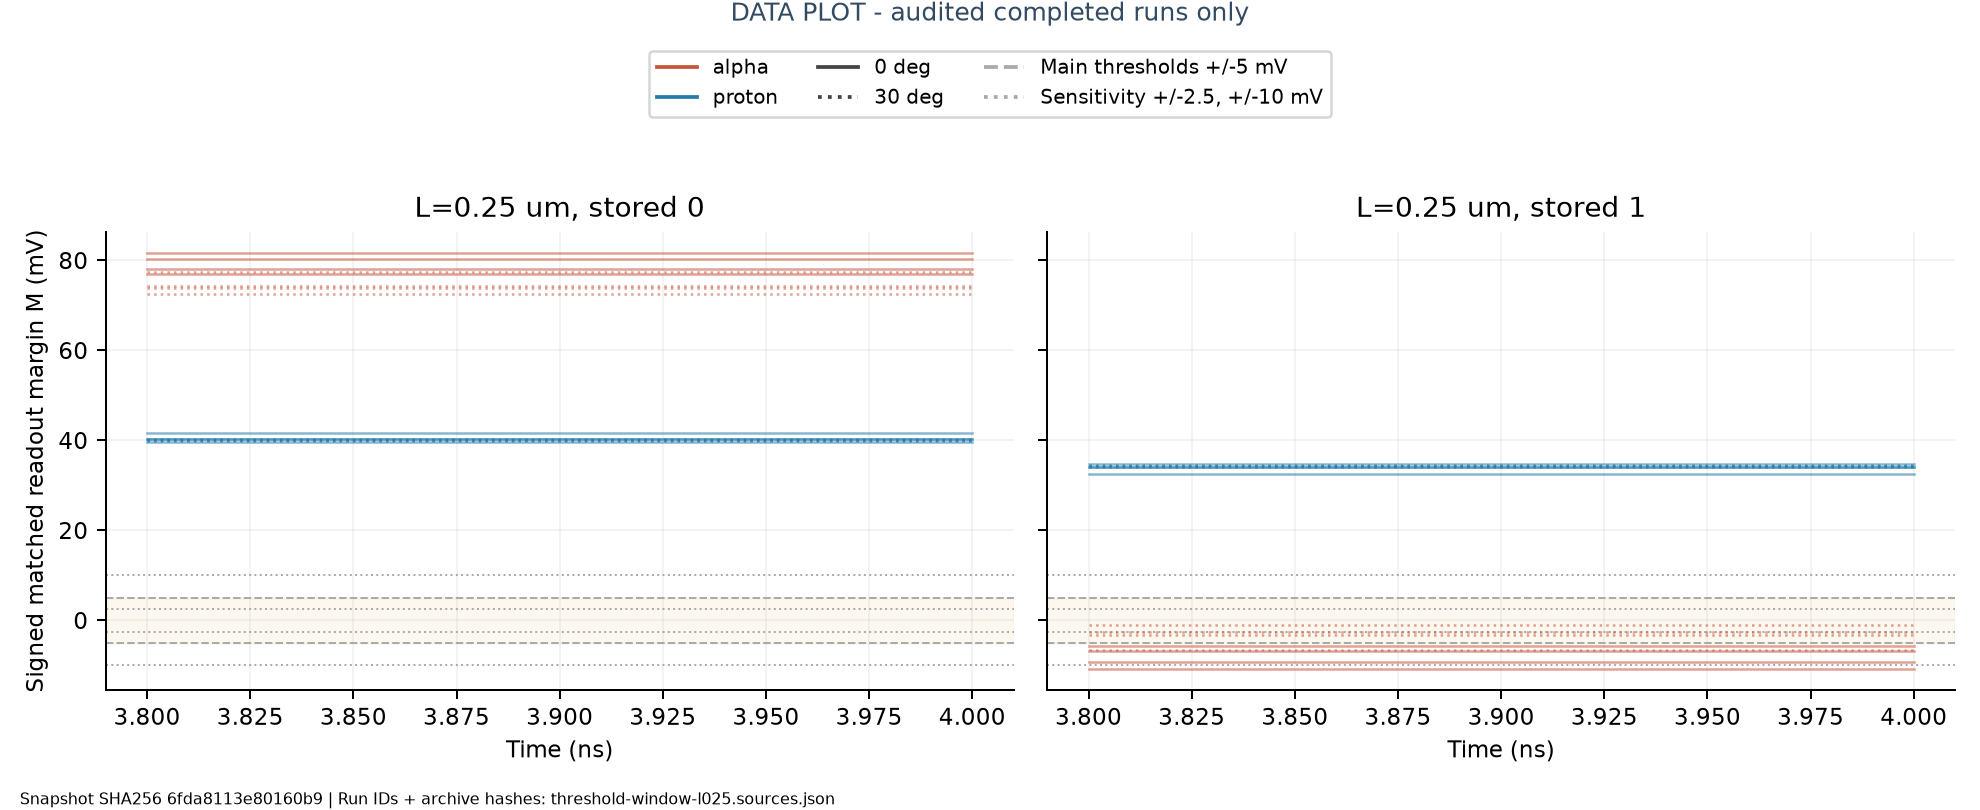
\includegraphics[width=0.48\textwidth]{figures/threshold-window-l025.png}
\caption{v3冻结设计下 0.18/0.25\um 的阈值与读窗敏感性。数据版本：20261012T0033Z-full；v4 阈值须另按基准冻结。}
\label{fig:threshold-l018}
\end{figure}
\begin{figure}[htbp]
\centering
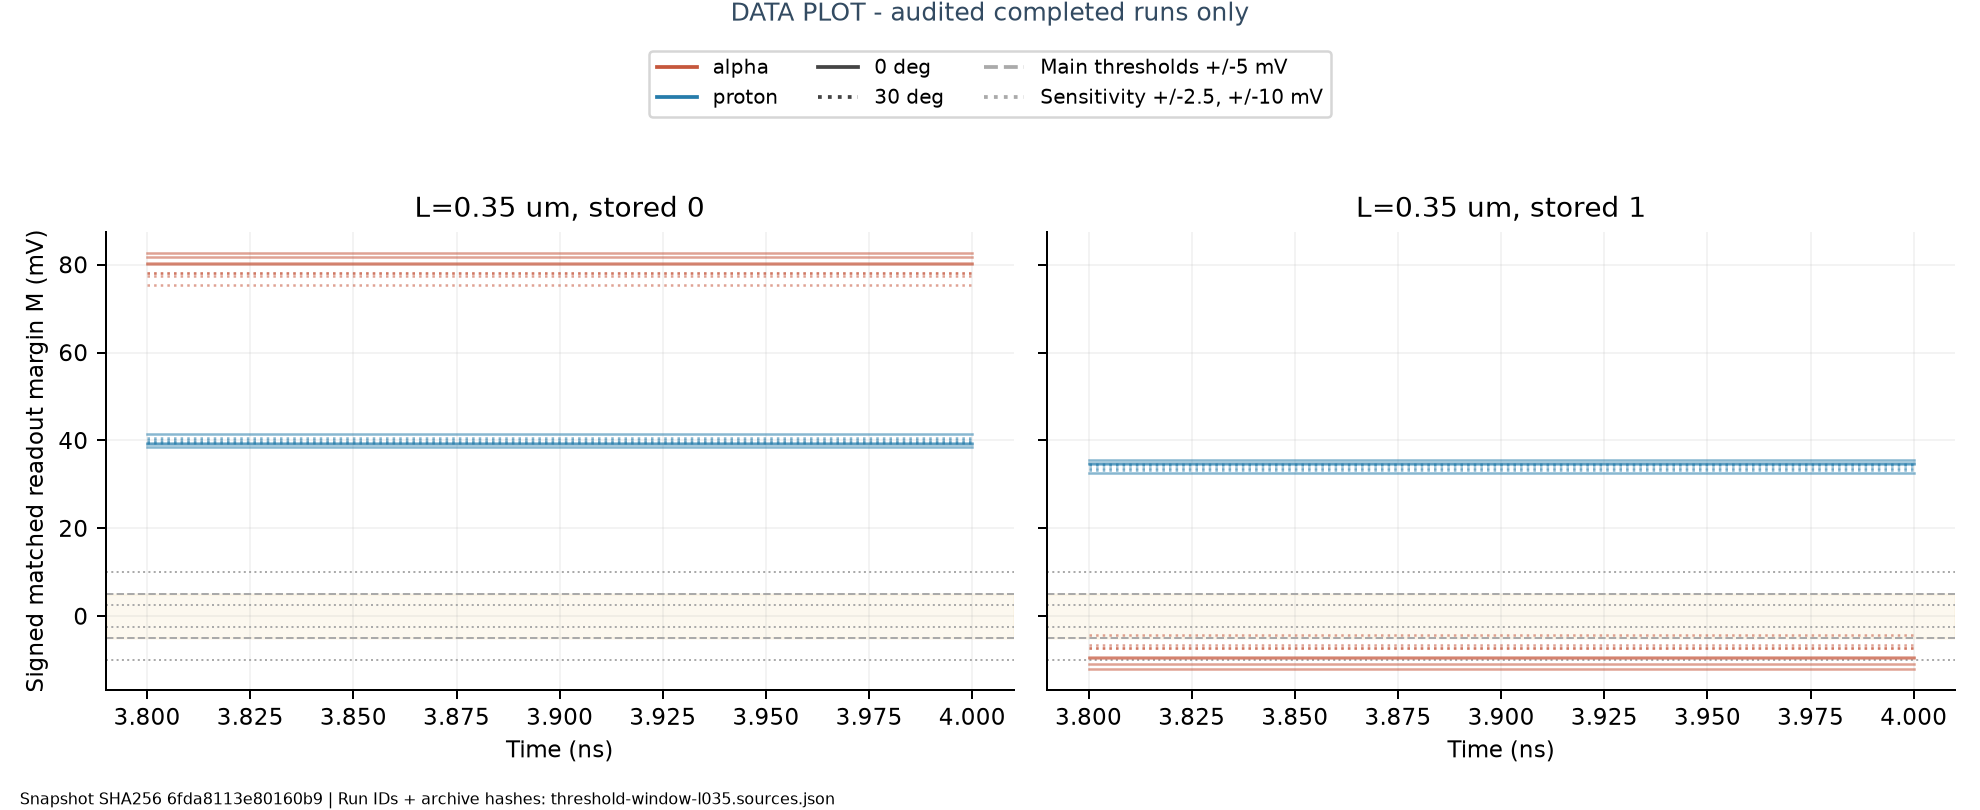
\includegraphics[width=0.48\textwidth]{figures/threshold-window-l035.png}
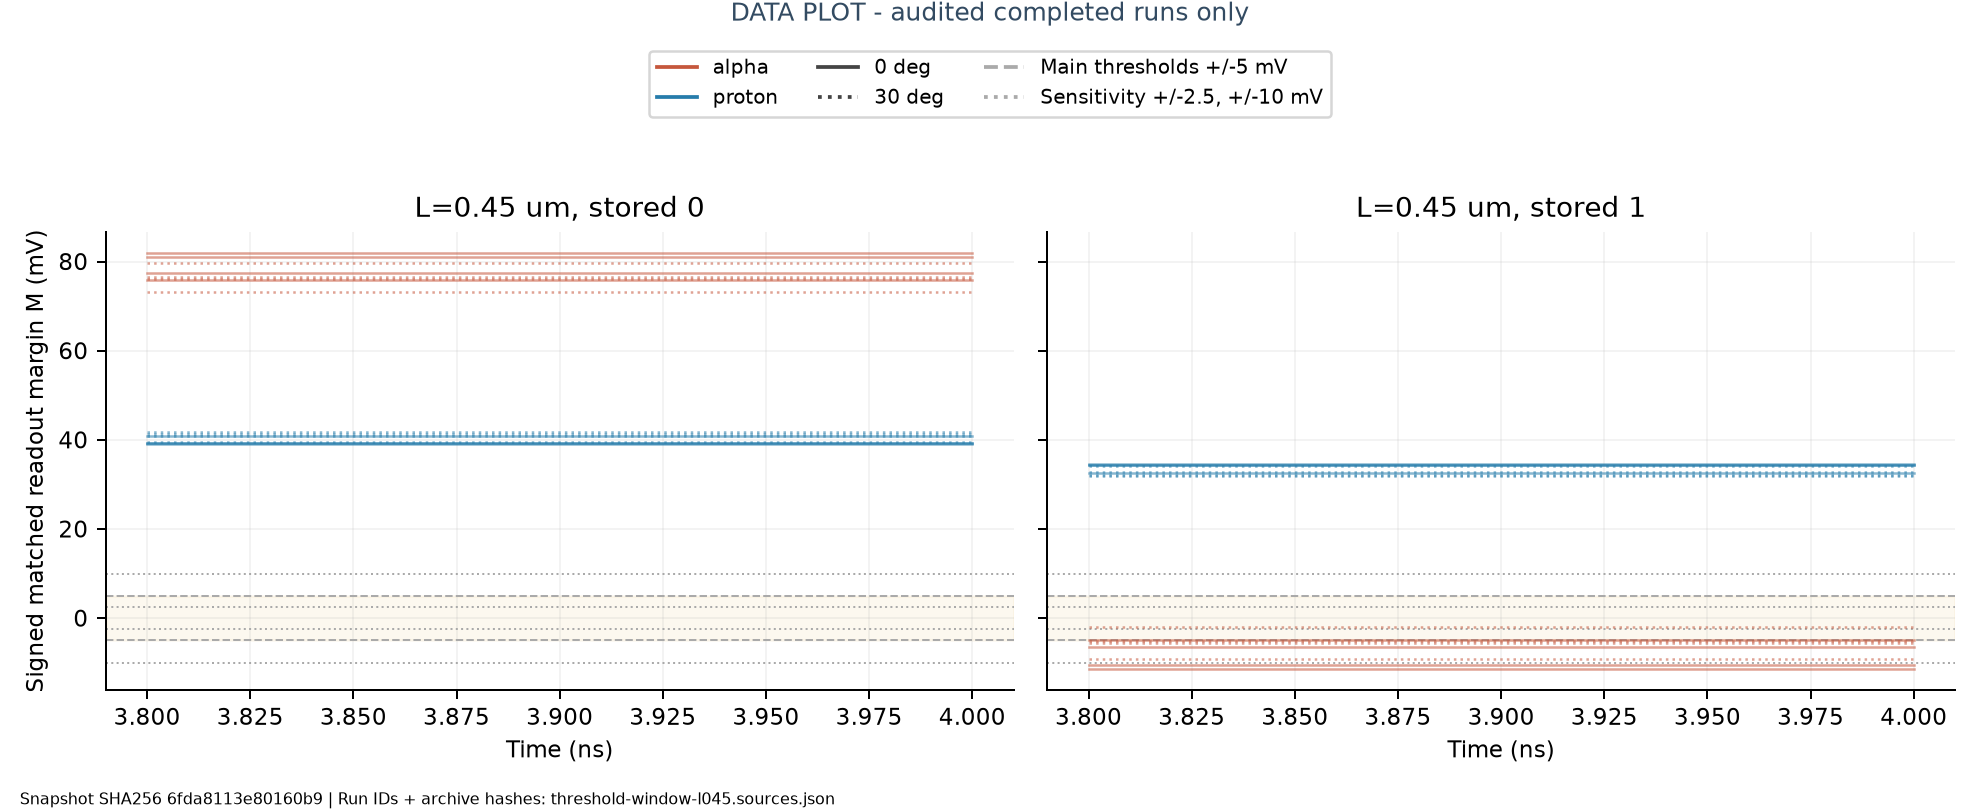
\includegraphics[width=0.48\textwidth]{figures/threshold-window-l045.png}
\caption{v3冻结设计下 0.35/0.45\um 的阈值与读窗敏感性。数据版本：20261012T0033Z-full。}
\label{fig:threshold-l045}
\end{figure}

\subsection{氧化层厚度局部敏感性}

图\ref{fig:oxide} 为固定事件 4/5/6\,nm 氧化层对照：最大变化约 0.11256\mV / 0.00578\fC，小于原容差，不宣称显著工艺效应；属于固定事件局部分析，不扩展为统计规律。

\begin{figure}[htbp]
\centering
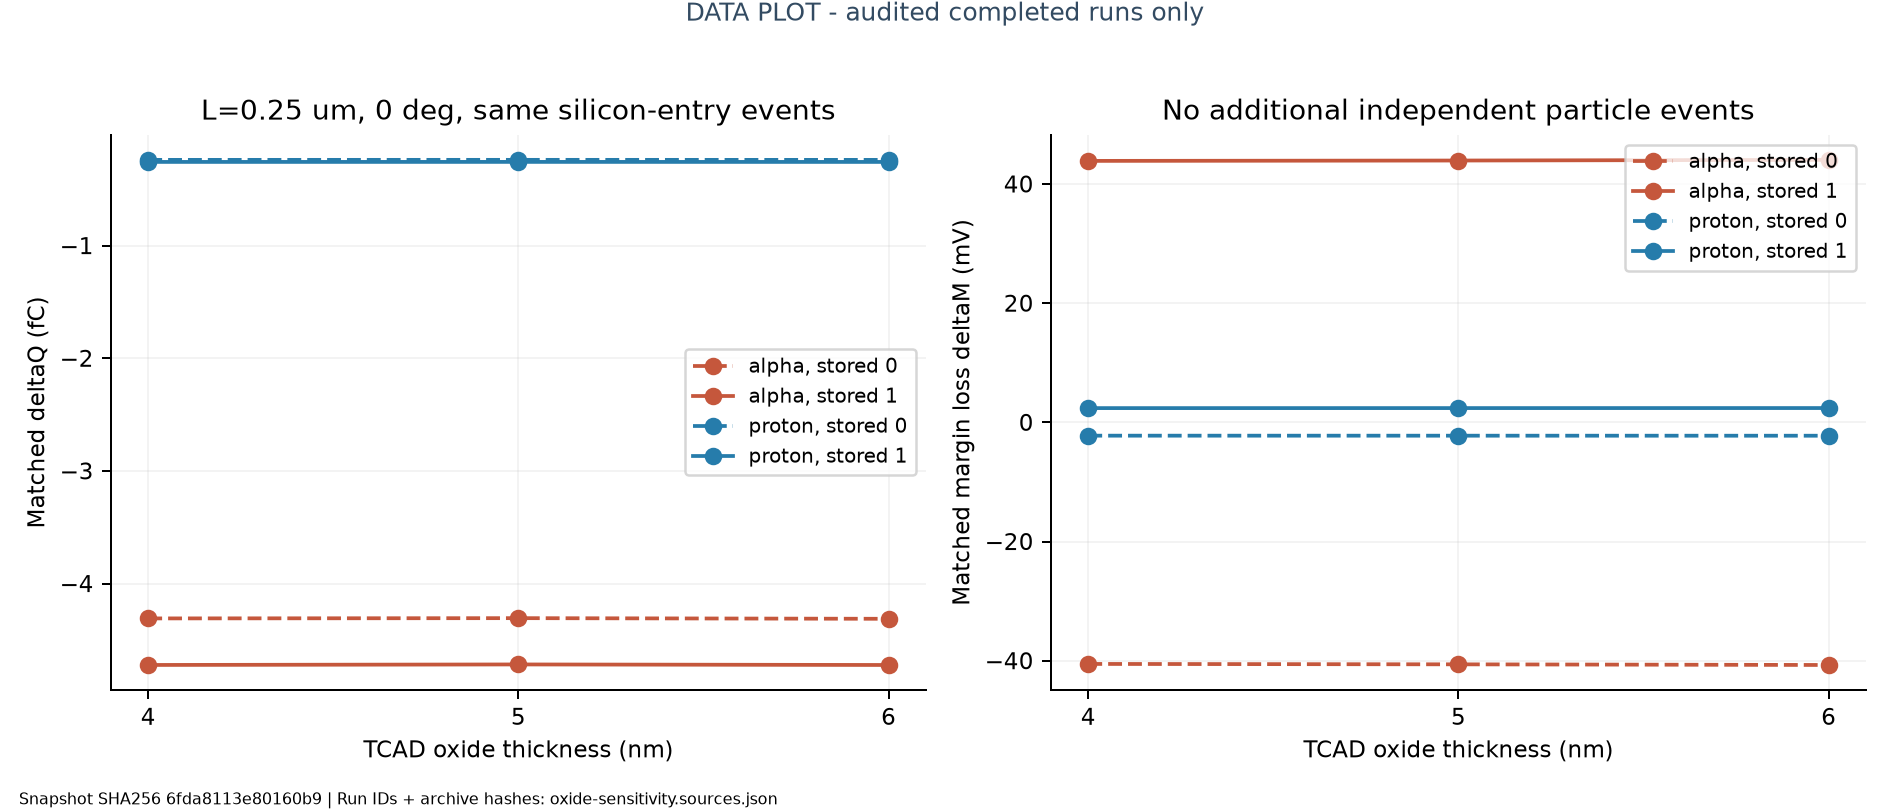
\includegraphics[width=0.7\textwidth]{figures/oxide-sensitivity.png}
\caption{v3冻结设计下 4/5/6\,nm 氧化层固定事件局部敏感性；最大变化约 0.11256\mV/0.00578\fC，小于容差。数据版本：20261012T0033Z-full。}
\label{fig:oxide}
\end{figure}

\subsection{历史预测基线：域内/域外误差}

图\ref{fig:residuals} 与表\ref{tab:pred-dm}--\ref{tab:pred-dq} 给出四个岭回归模型在原冻结划分下的预测残差与误差（域内 $\Delta M$ MAE 约 0.53--0.55\mV）。旧冻结划分；$Q_{dep}$ 等特征依赖 Geant4，推理成本不能省略输运；该基线不冒充新模型的独立盲测。

\begin{figure}[htbp]
\centering
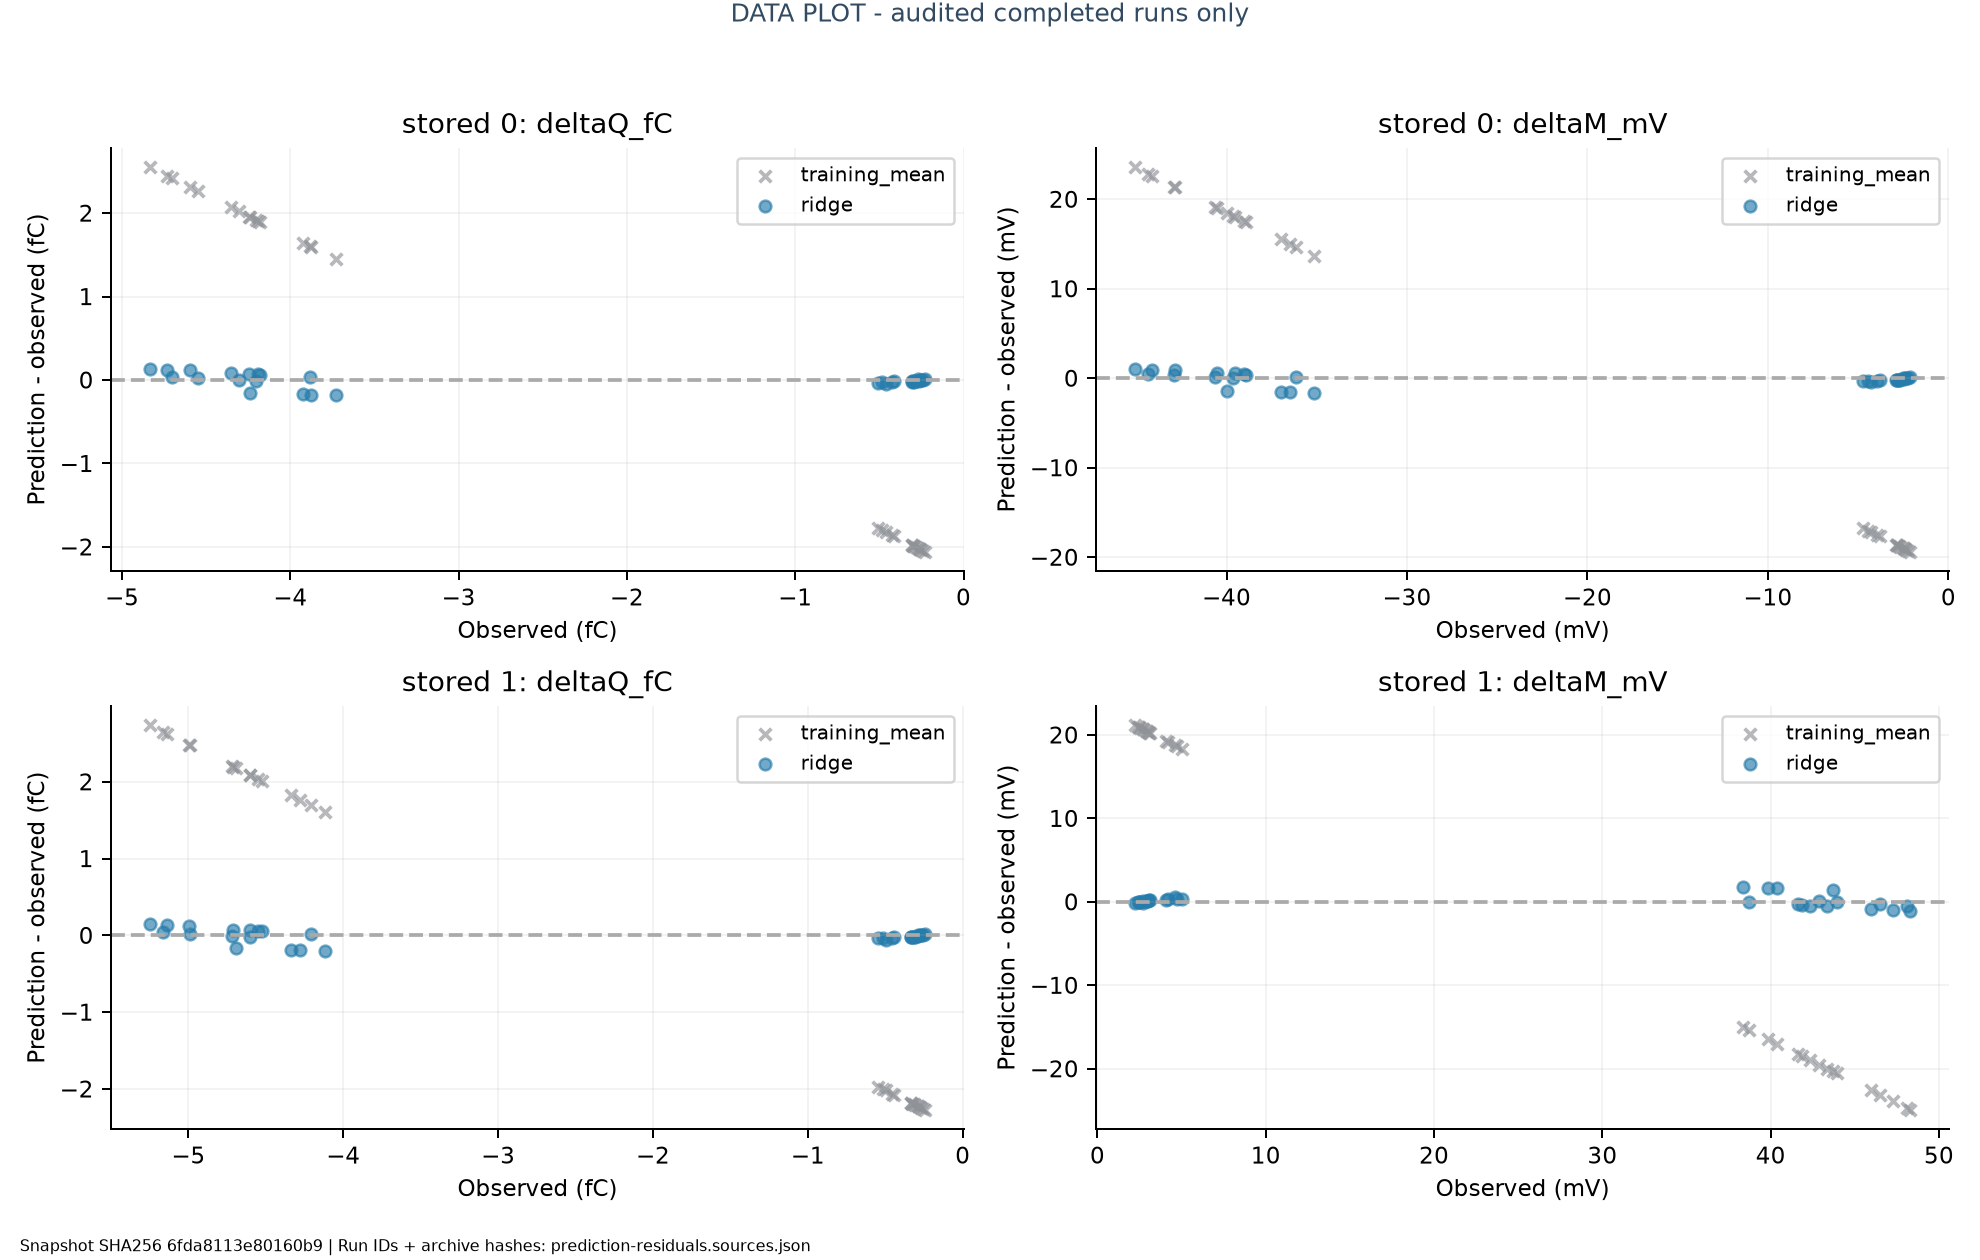
\includegraphics[width=0.75\textwidth]{figures/prediction-residuals.png}
\caption{v3冻结设计下岭回归与均值基线的预测残差（域内/域外、两目标）；旧冻结划分，特征含 Geant4 沉积。数据版本：20261012T0033Z-full。}
\label{fig:residuals}
\end{figure}
\begin{table}[htbp]
\centering\small
\caption{裕量预测误差（mV），按 bit、域内/域外与模型分开}
\label{tab:pred-dm}
\begin{tabular}{lllrrrrrr}
\toprule
集合 & 位 & 模型 & $n$ & 缺失 & 无效 & MAE & RMSE & 最大误差\\
\midrule
留出 & 0 & 均值基准 & 16 & 0 & 0 & 18.320612 & 18.448022 & 22.860163\\
留出 & 0 & 岭回归 & 16 & 0 & 0 & 0.526964 & 0.798415 & 1.645649\\
留出 & 1 & 均值基准 & 16 & 0 & 0 & 19.936695 & 20.066626 & 24.741705\\
留出 & 1 & 岭回归 & 16 & 0 & 0 & 0.549768 & 0.838043 & 1.765441\\
外推 & 0 & 均值基准 & 16 & 0 & 0 & 18.742144 & 18.867683 & 23.569637\\
外推 & 0 & 岭回归 & 16 & 0 & 0 & 0.404964 & 0.519434 & 1.075289\\
外推 & 1 & 均值基准 & 16 & 0 & 0 & 20.091257 & 20.219896 & 24.915029\\
外推 & 1 & 岭回归 & 16 & 0 & 0 & 0.387723 & 0.504929 & 1.105078\\
\bottomrule
\end{tabular}

\end{table}
\begin{table}[htbp]
\centering\small
\caption{电荷预测误差（fC），不与 mV 混合平均}
\label{tab:pred-dq}
\begin{tabular}{lllrrrrrr}
\toprule
集合 & 位 & 模型 & $n$ & 缺失 & 无效 & MAE & RMSE & 最大误差\\
\midrule
留出 & 0 & 均值基准 & 16 & 0 & 0 & 1.942616 & 1.956036 & 2.416036\\
留出 & 0 & 岭回归 & 16 & 0 & 0 & 0.056607 & 0.088294 & 0.181592\\
留出 & 1 & 均值基准 & 16 & 0 & 0 & 2.140865 & 2.154850 & 2.651122\\
留出 & 1 & 岭回归 & 16 & 0 & 0 & 0.061766 & 0.094644 & 0.198945\\
外推 & 0 & 均值基准 & 16 & 0 & 0 & 2.011262 & 2.025386 & 2.548969\\
外推 & 0 & 岭回归 & 16 & 0 & 0 & 0.052826 & 0.068049 & 0.136393\\
外推 & 1 & 均值基准 & 16 & 0 & 0 & 2.183932 & 2.198297 & 2.733561\\
外推 & 1 & 岭回归 & 16 & 0 & 0 & 0.051740 & 0.067155 & 0.144228\\
\bottomrule
\end{tabular}

\end{table}

\subsection{原生软件窗口证据}

图\ref{fig:native-phys}（左、右两幅）为完整原生窗口（非裁切）：保留图例、单位与坐标轴定义（Abs(ElectricField-V)，V/cm；SVisual 竖向 X/横向 Y）。F01--F13 为真实数据生成的 DATA PLOT，本两图才是原生窗口证据。

\begin{figure}[htbp]
\centering
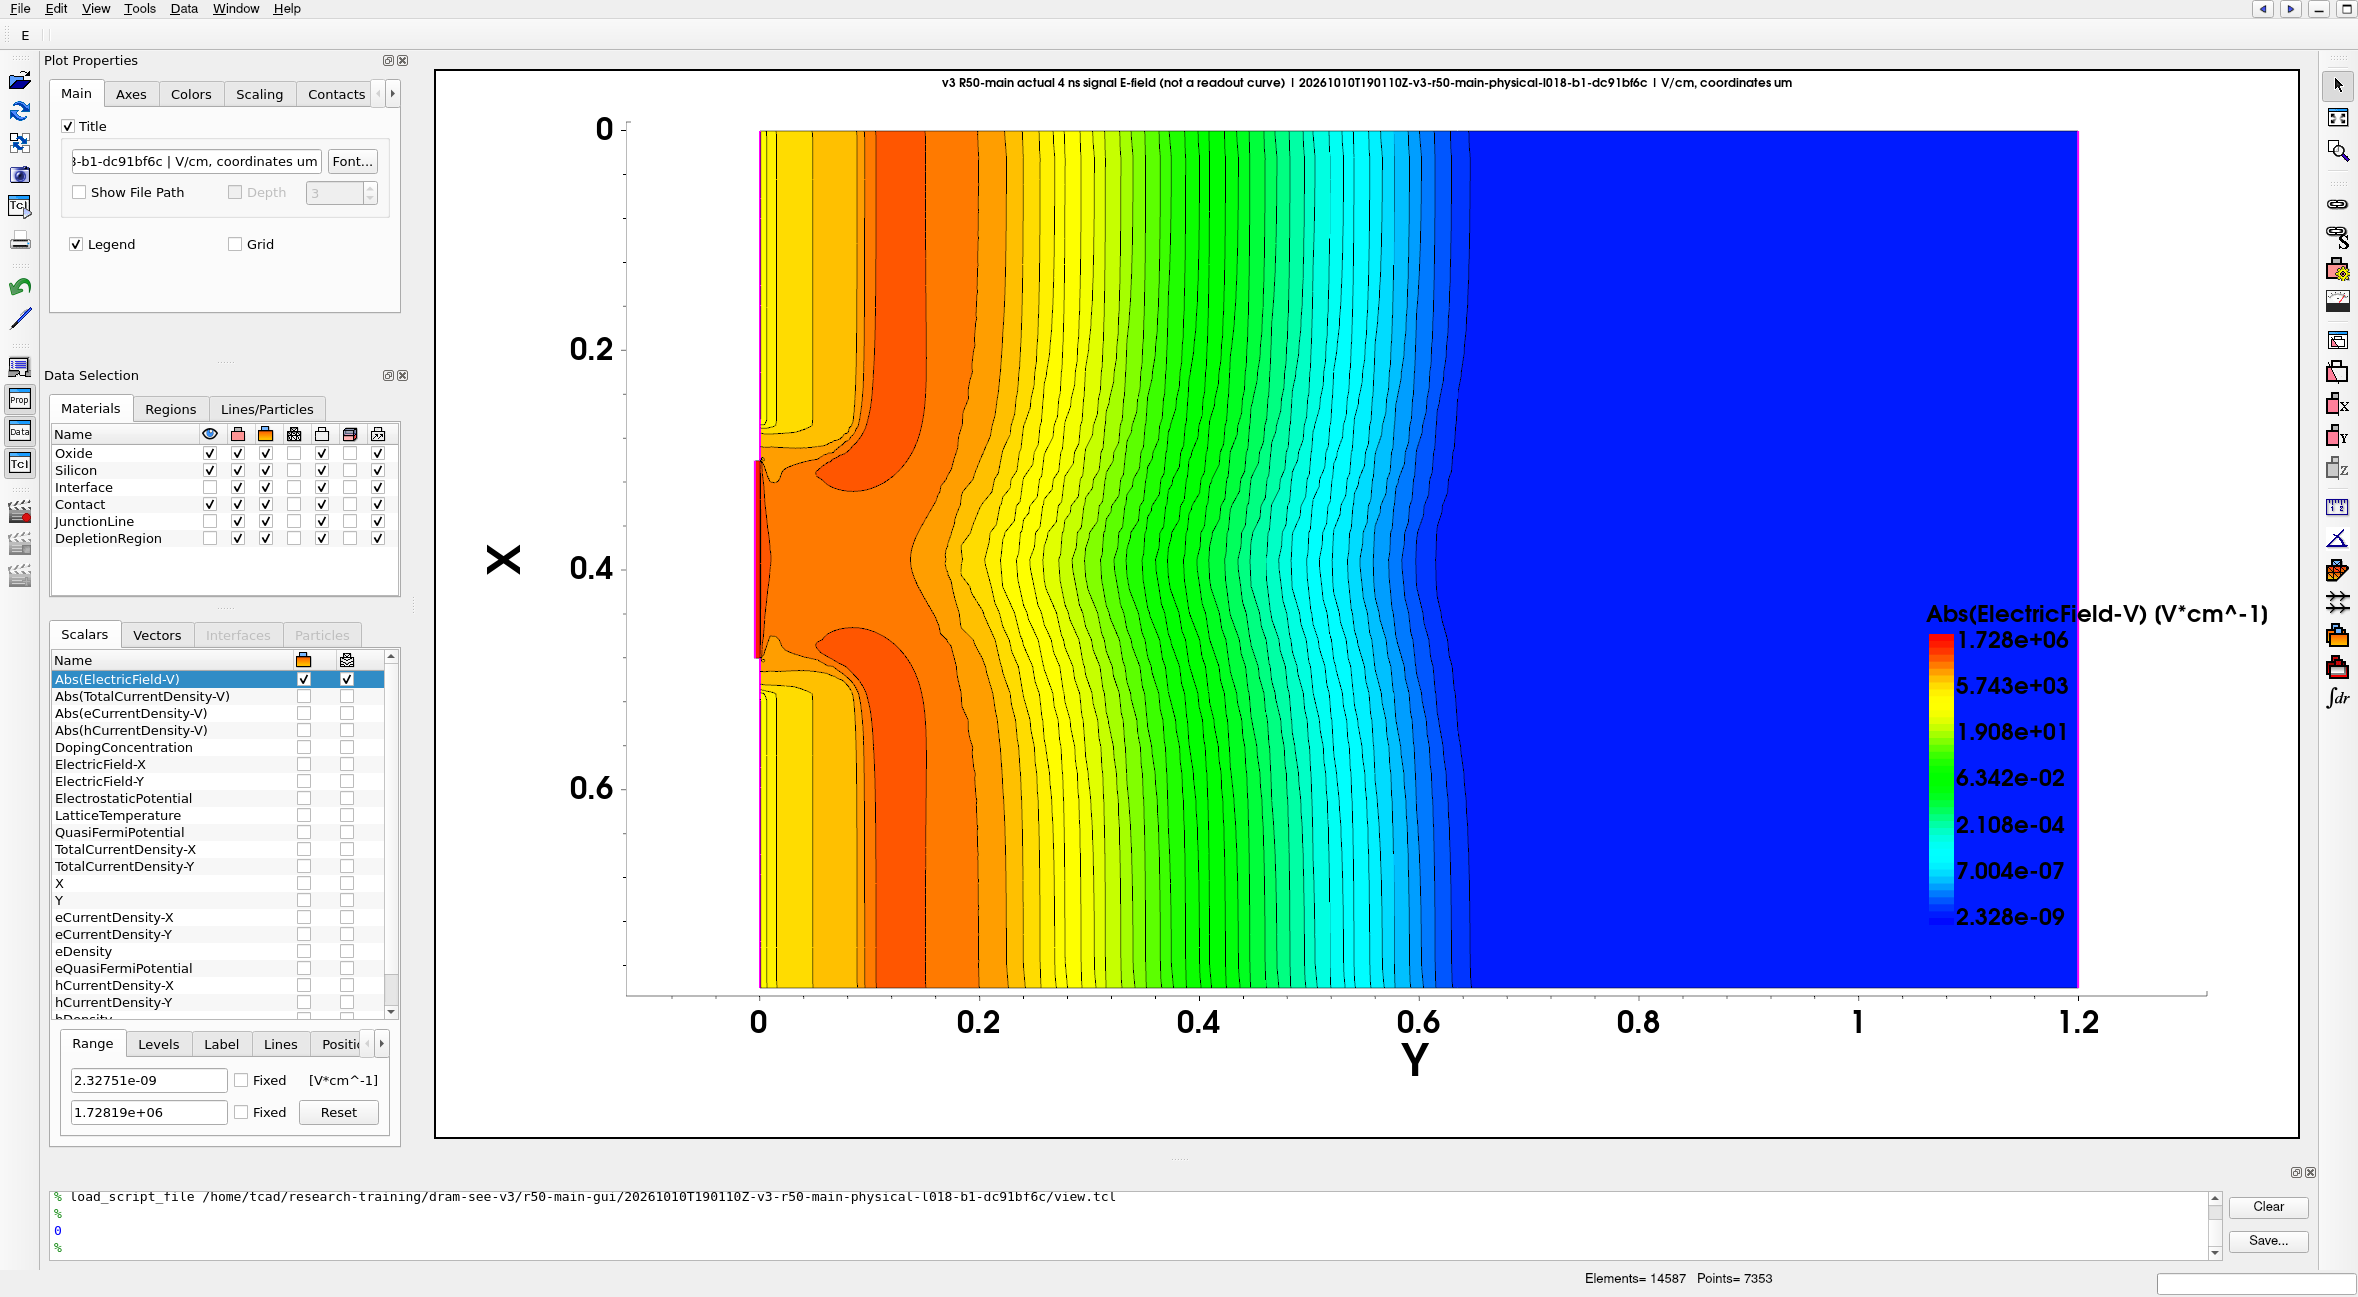
\includegraphics[width=0.48\textwidth]{figures/native-physical-window.png}
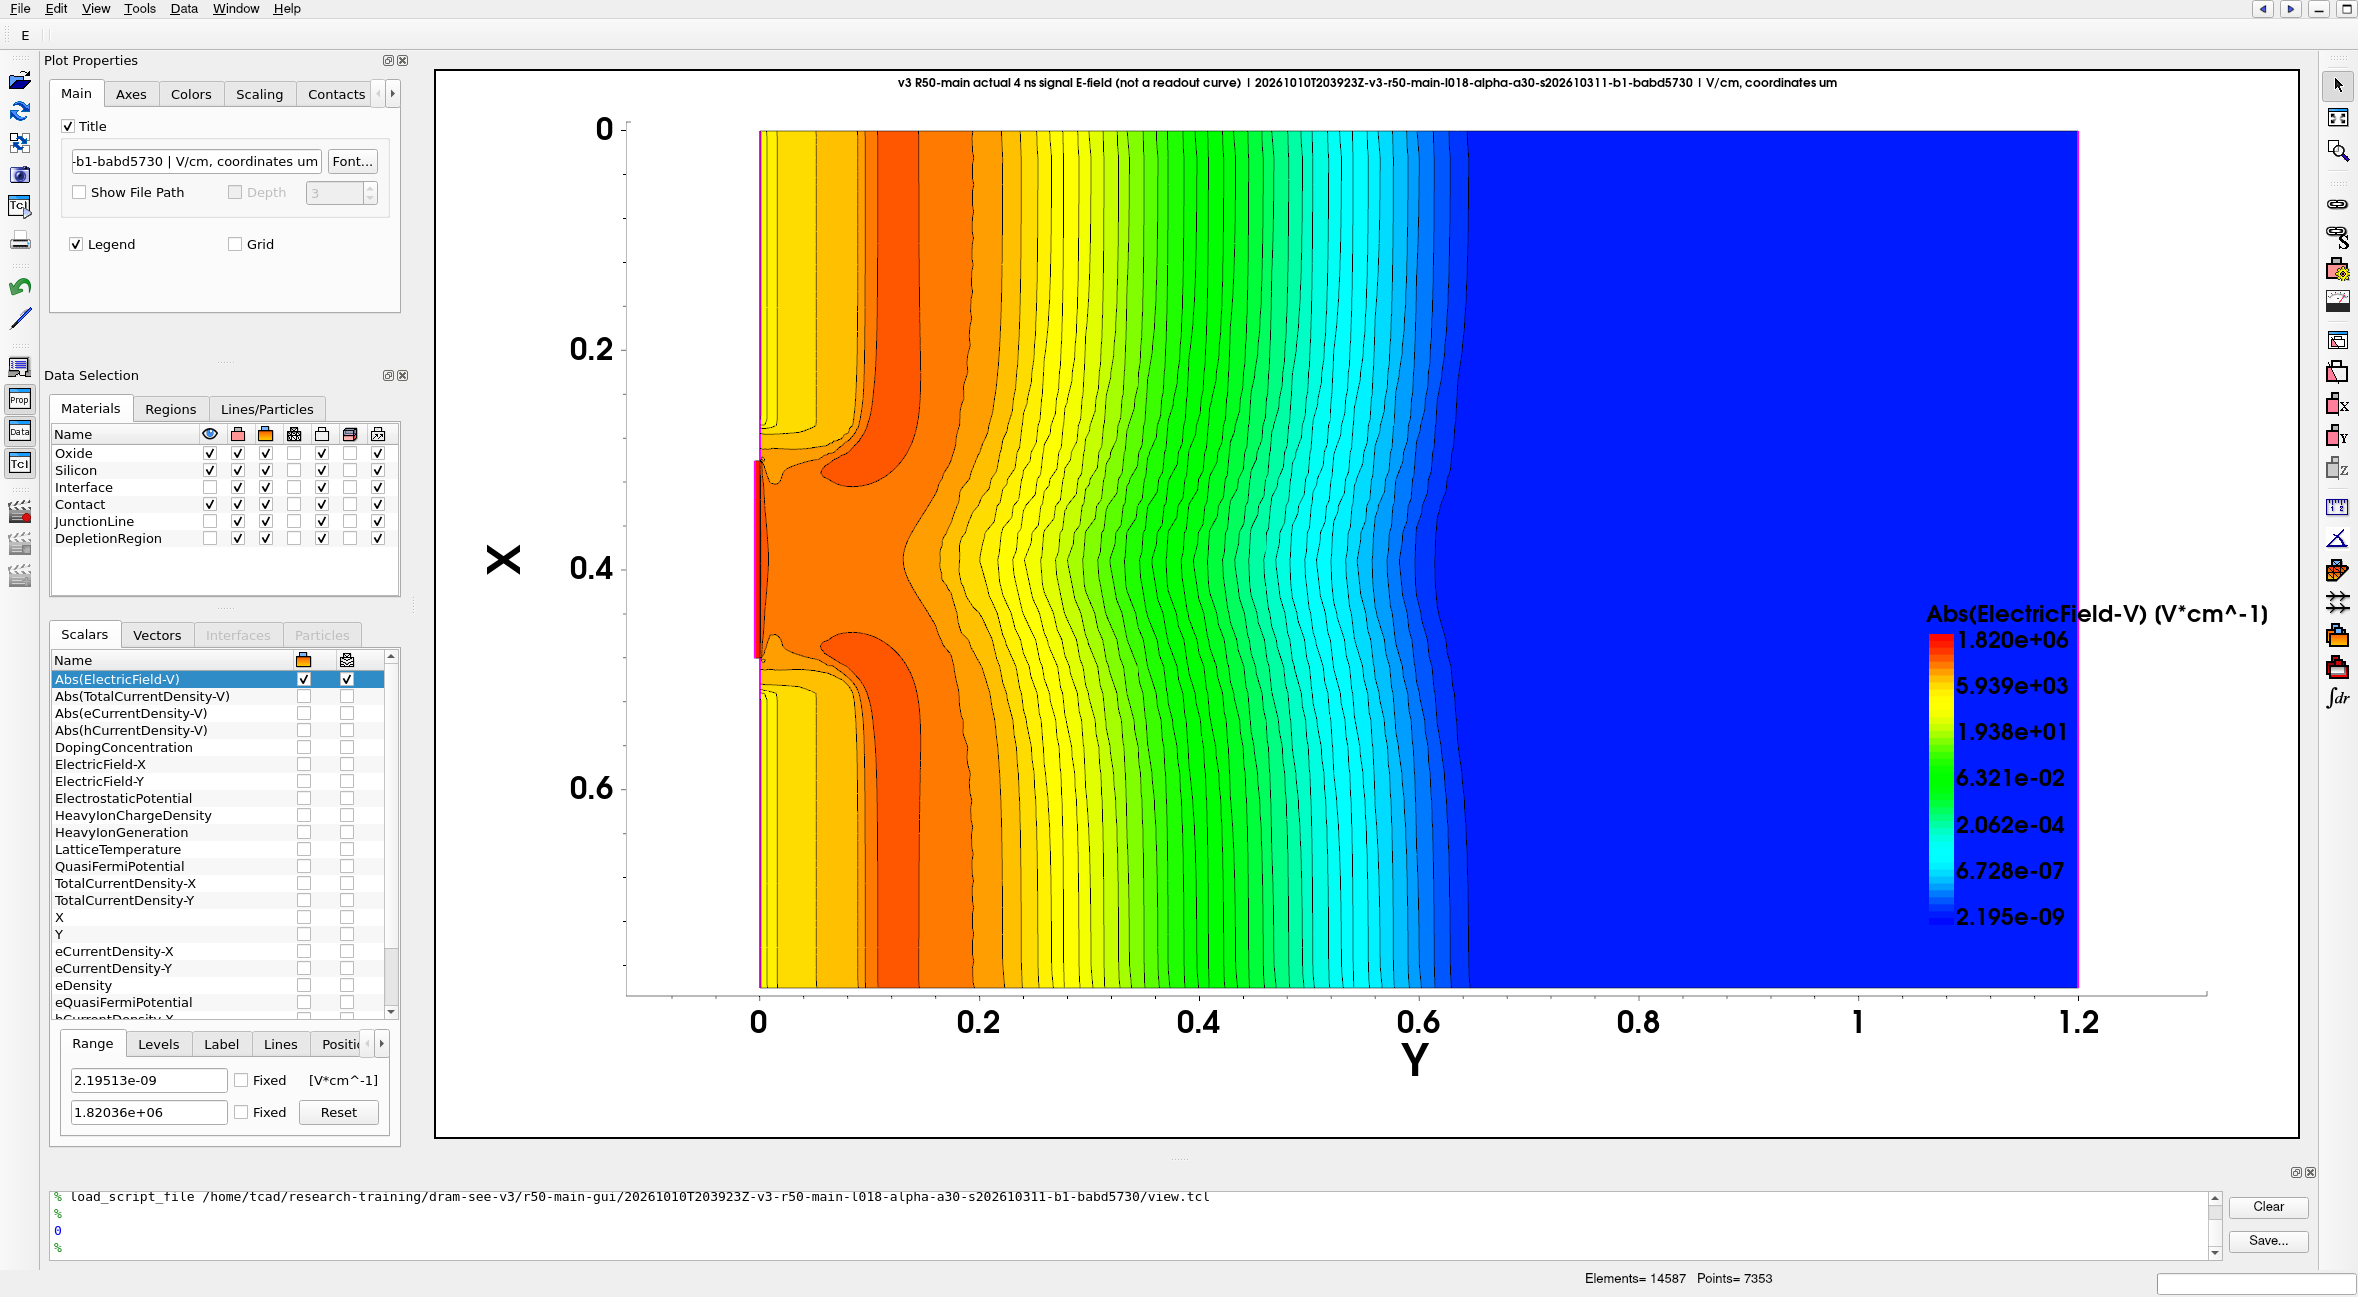
\includegraphics[width=0.48\textwidth]{figures/native-event-window.png}
\caption{v3原生模型/场分布窗口（左）与指定事件 4\ns 电场分布（右）；Abs(ElectricField-V)，V/cm，勿擅自换轴。数据版本：20261012T0033Z-full。}
\label{fig:native-phys}
\end{figure}

\subsection{待补：r0.6 新结果与成本统计}

\textbf{待补。} D0--D3 第一波合格结果、吞吐/资源图（单/双/三任务）、v4 两 bit 全周期与 KCL、α/质子源资格图、数据覆盖矩阵、AI 消融与分组 CV、截面/外部对比——先有合格数据再画图，清单见 \texttt{materials/图表引用清单.md} 的"下一批待补图"。
